\chapter{Webové aplikace pro zpřístupnění digitalizovaných archiválií}
 \label{chap:archives}
V této sekci jsou představeny aktuálně používané systémy jednotlivých archivů, které zpřístupňují digitalizované archiválie. Následně bude provedeno porovnání jednotlivých prohlížečů snímků archiválií, vyhodnoceny budou jak jejich klady, tak i~zápory. Dále budou porovnány technologie, na nichž jsou dané systémy postaveny, a~zda se vždy jedná o řešení na míru nebo společně sdílí nějaké aplikační jádro.

\section{Národní archiv}
Národní archiv má vlastní elektronickou badatelnu \href{https://vademecum.nacr.cz/vademecum}{Vademecum}\footnote{https://vademecum.nacr.cz/vademecum}, která veřejnosti poskytuje přístup ke sbírkám a~fondům spravovaných Národním archivem. V~rámci aplikace jsou spravovány archivní fondy, archivní pomůcky a~inventární záznamy. Aplikace umožňuje v~daných archiváliích vyhledávat pomocí více kritérií jako například pomocí rejstříku, časového období či podle toho, zda daná archiválie obsahuje zdigitalizované přílohy. 

\begin{figure}[htbp]
\centering
    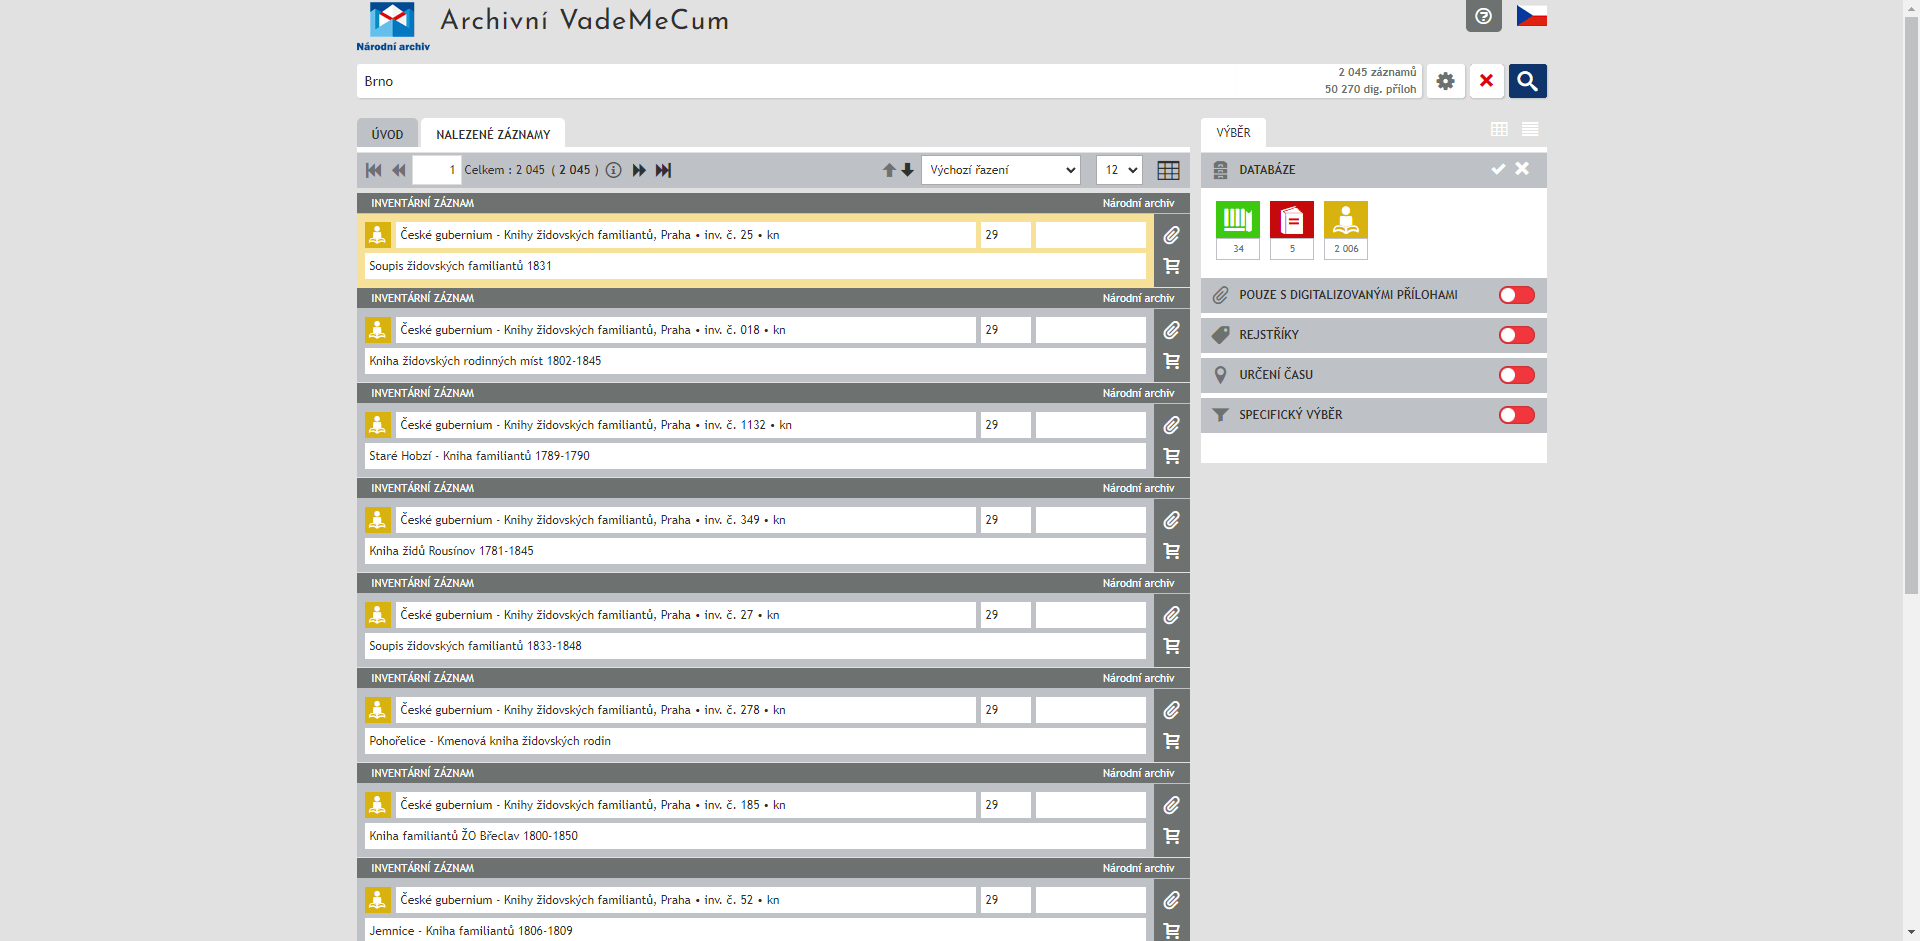
\includegraphics[scale=.2]{obrazky-figures/archives/hpPraha/vyhledani.png}
    \caption{Vyhledávání archiválií v~systému Národního archivu}
\end{figure}
\noindent
Podle analýzy zdrojového kódu to vypadá, že aplikace běží na Apache/2.4.54, které je hostované na systému Debian. Požadavek na vyhledání se posílá na SearchBean, což díky jmenným konvencím naznačuje, že serverová část aplikace je napsána v~Javě. V~rámci analýzy zdrojového kódu byly nalezeny čitelné komentáře, což naznačuje, že kód byl tvořen ručně a~podle odkazů (například \texttt{header.jspf}) to vypadá, že pro klientskou část aplikace se využívá technologie Java Server Pages. Z toho vyplývá, že celá aplikace je napsána v~Javě a~nevyužívá architekturu, kde by zobrazovací logika byla oddělena a~komunikovala pomocí API. Na klientské části se dále vyskytují JavaScriptové knihovny jako jQuery a~Zoomify pro prohlížení archiválií.
\newpara
Prohlížeč archiválií má dobrý poměr mezi ovládacími prvky a~plochou pro zobrazení archiválie. Mezi archiváliemi se lze orientovat a navigovat pomocí postranního menu s~náhledy nebo pomocí horního navigačního menu. Aplikace podporuje klávesové zkratky a~umožňuje i~stažení snímku po vyplnění CAPTCHA. Aplikace dále umožňuje i~rotovat sken po  malém úhlu. Možnost resetovat nastavení a~vrátit snímek do původní pozice zde chybí.

\begin{figure}[htbp]
\centering
    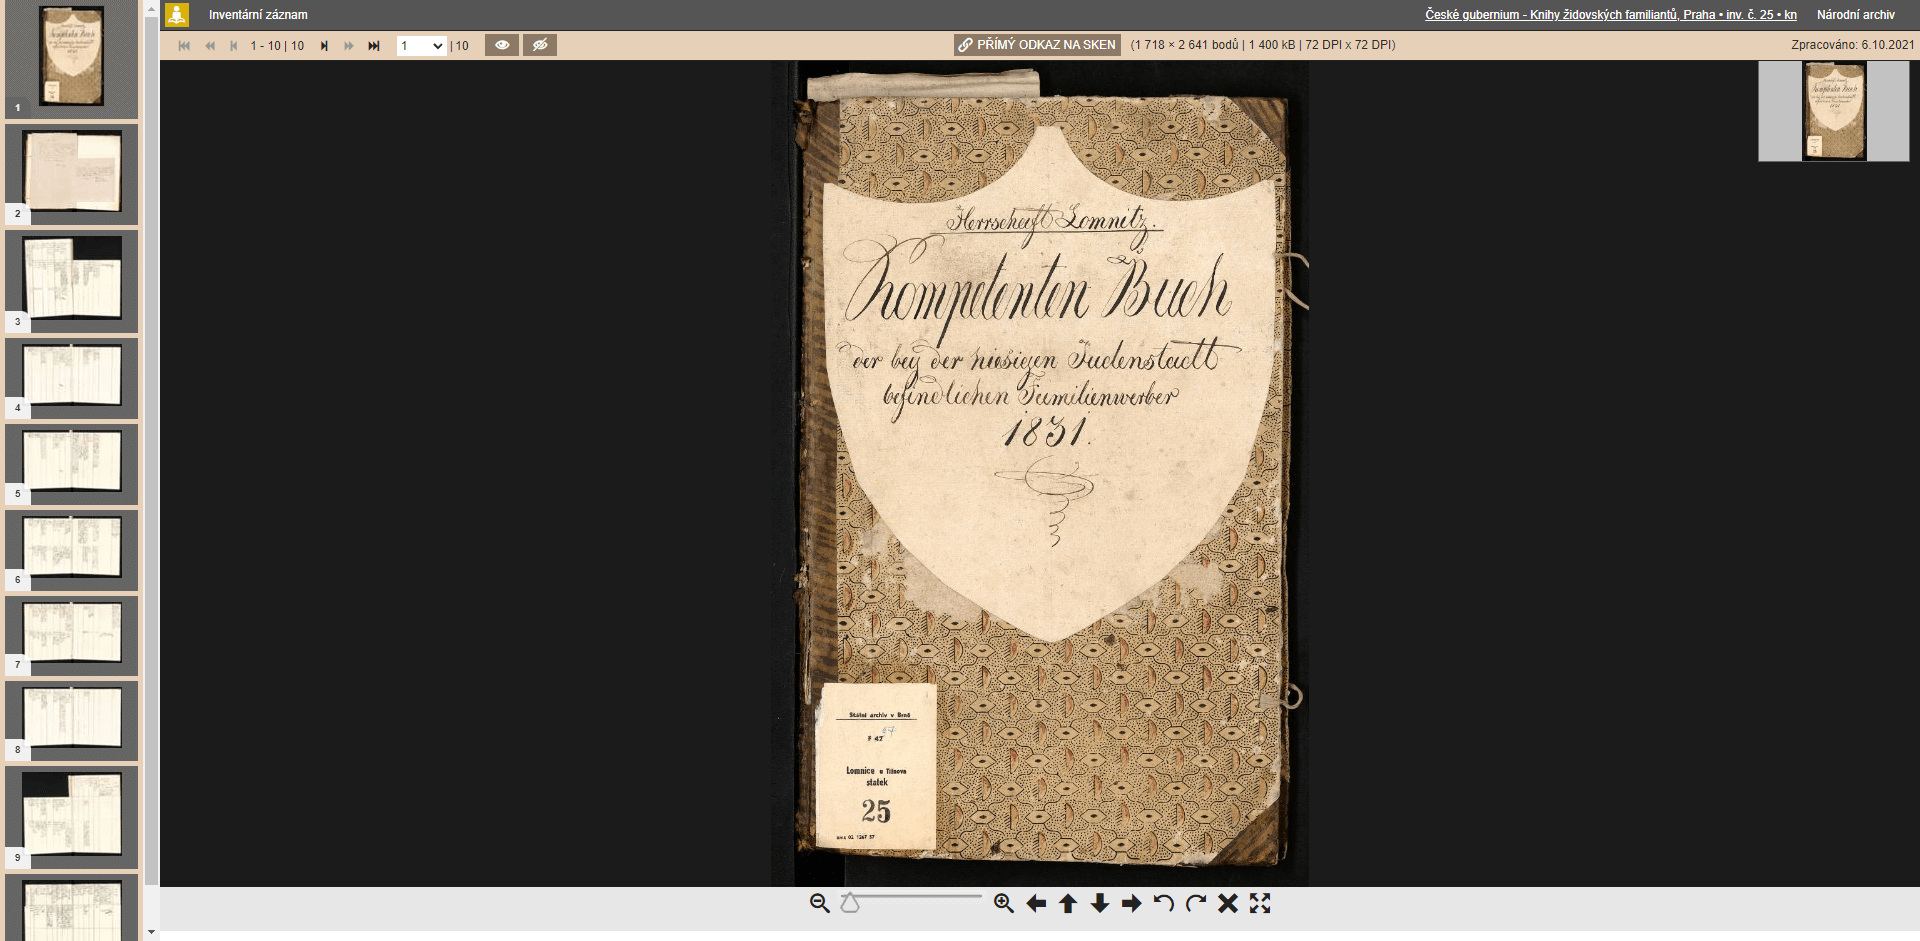
\includegraphics[scale=.2]{obrazky-figures/archives/hpPraha/prohlizec.png}
    \caption{Prohlížeč archiválií v~systému Národního archivu}
\end{figure}

\section{Moravský zemský archiv}
Moravský zemský archiv své matriční knihy badatelům zpřístupňuje na portálu \href{https://www.mza.cz/actapublica/matrika/hledani}{Actapublica}\footnote{https://www.mza.cz/actapublica/matrika/hledani}. Jednotlivé matriky lze vyhledávat například podle obce, původce nebo čísla knihy. Vyhledávač obcí je doplněn o našeptávání okresů, což umožňuje vybrat správnou obec při shodě jmen mezi obcemi.

\begin{figure}[htbp]
\centering
    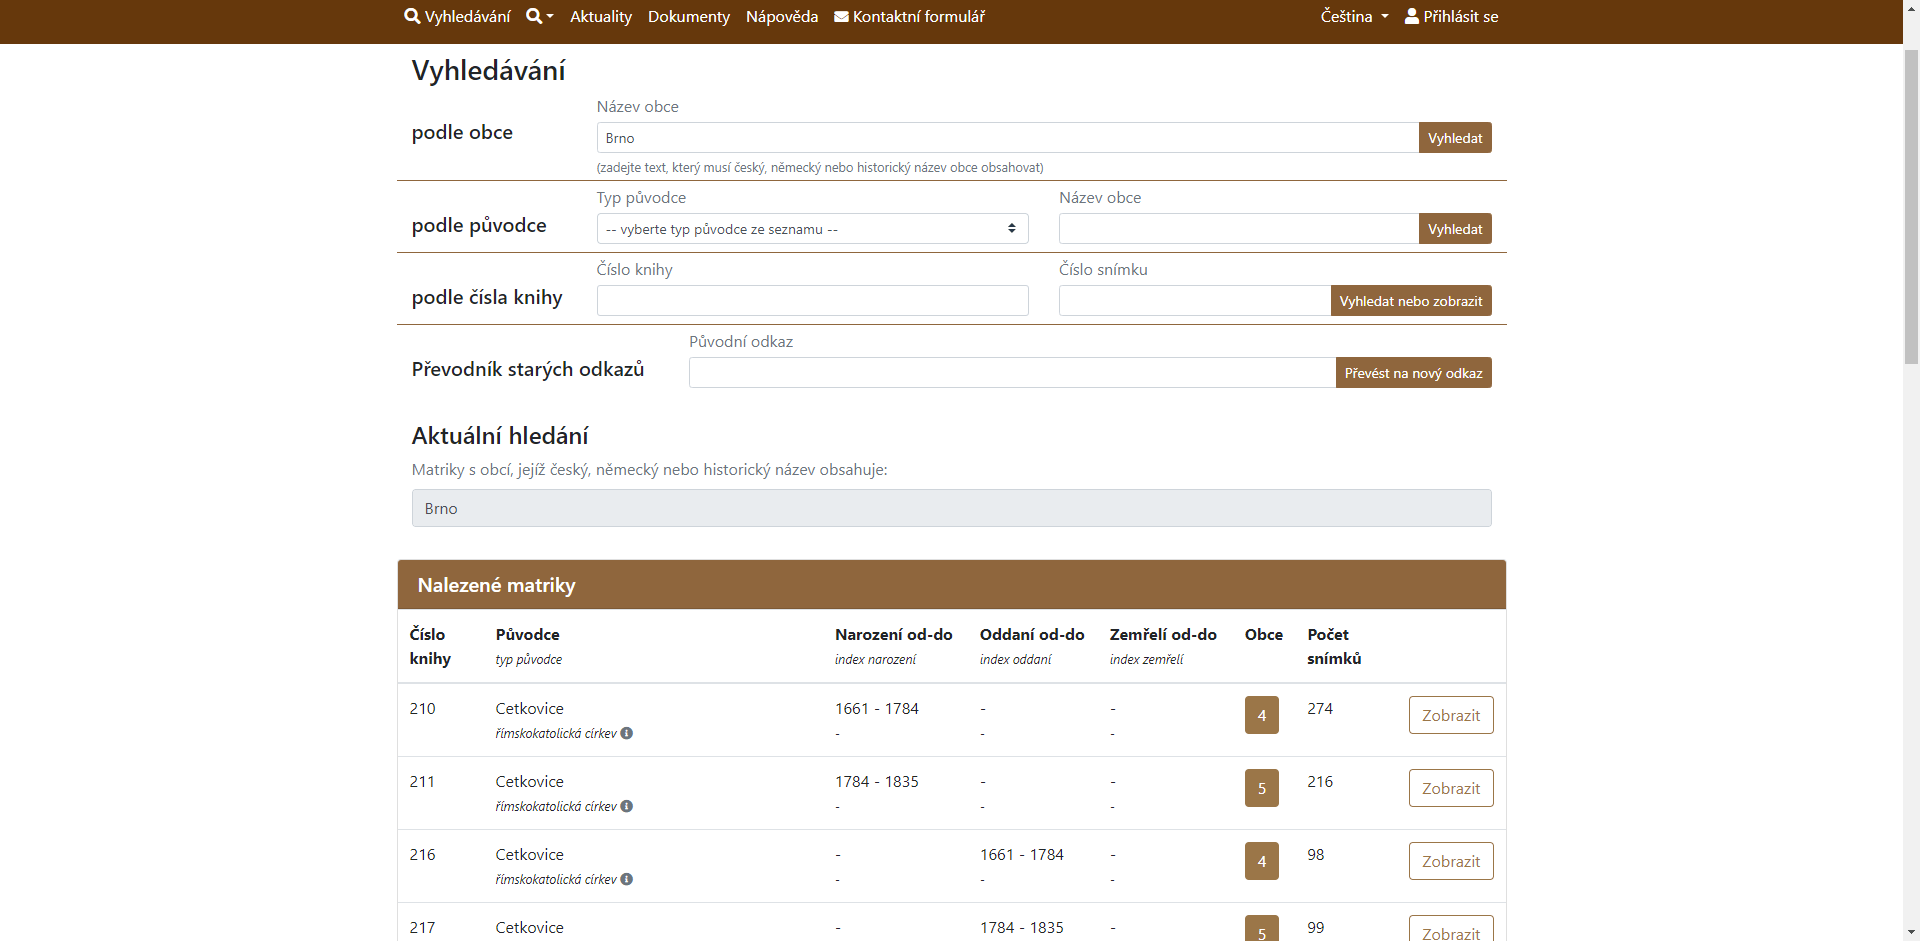
\includegraphics[scale=.2]{obrazky-figures/archives/mza/vyhledani.png}
    \caption{Vyhledávání archiválií v~systému Moravského zemského archivu}
\end{figure}
\newpage

\noindent
Podle analýzy komunikace, kde se odesílá ASP.NET\_SessionId, lze předpokládat, že aplikace běží na dotnetu s~knihovnou ASP.NET. Nástrojem WhatRuns bylo identifikováno běhové prostředí IIS 7.5 na Windows serveru. Podle struktury volání, kde se vrací celé HTML soubory obsahující čitelné komentáře, lze usoudit, že obdobně jako u~Národního archivu se zde jedná o~monolitickou aplikaci, která řeší jak aplikační logiku, tak zobrazování. Aplikace pravděpodobně běží na aplikačním rámci ASP.NET MVC. V klientské části aplikace využívá JavaScriptové knihovny jako jQuery, Bootstrap a~Popper.JS. Architektura je totožná s~předchozím archivním systémem. Pro zobrazování archiválií používá knihovnu \href{https://openseadragon.github.io/}{OpenSeaDragon}\footnote{https://openseadragon.github.io} a~jako formát skenů používá Deepzoom.
\newpara
 Prohlížeč archiválií je vybaven kvalitním režimem celé obrazovky a je zde možné zobrazit archiválii přes celé okno. Aplikace nenabízí náhled dalších snímků a~navigace po archiválii je tedy možná pouze pomocí horního navigačního menu. Aplikace umožňuje rotaci archiválie o 90° a nastavení jasu a~kontrastu pro lepší čitelnost archiválie. Kladně hodnotím záložky v~rámci archiválie pro snazší vyhledávání. Aplikace nenabízí možnost stáhnutí snímku v~plné kvalitě. Není sice odchycen event na canvasu, který by samotné stažení znemožnil, ale použití formátu DeepZoom dělá výsledný stažený snímek dále nepoužitelný. 

\begin{figure}[htbp]
\centering
    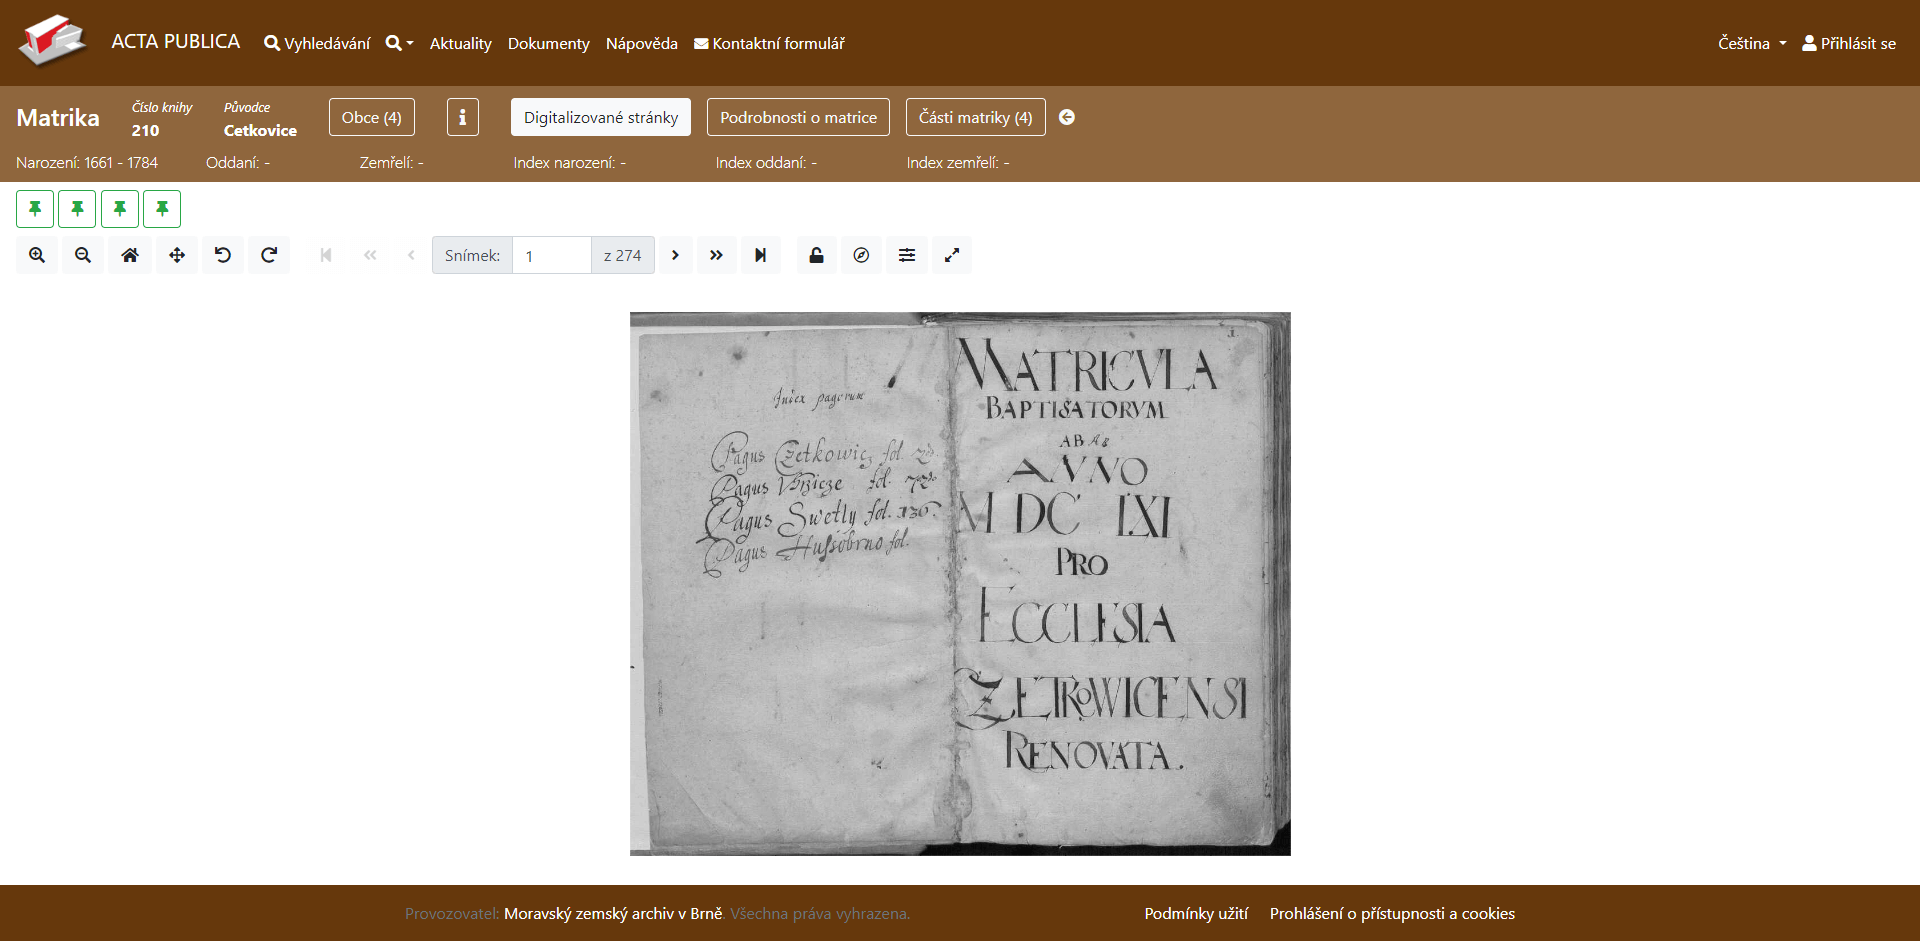
\includegraphics[scale=.2]{obrazky-figures/archives/mza/prohlizec.png}
    \caption{Prohlížeč archiválií v~systému Moravského zemského archivu}
\end{figure}
\newpage
\section{Zemský archiv v~Opavě}
Zemský archiv v~Opavě zpřístupňuje svůj \href{https://digi.archives.cz}{digitální archiv}\footnote{https://digi.archives.cz}, který má obdobné rozložení i~formát zobrazování dat jako Vademecum od Národního archivu. Navíc je zde možnost v~rámci filtrování vybrat typ archiválií, kde lze volit mezi matrikami, mapami, kronikami a~mnoha dalšími kategoriemi. V~rámci archiválií se vyhledává pomocí jednoho plně textového vyhledávače.

\begin{figure}[htbp]
\centering
    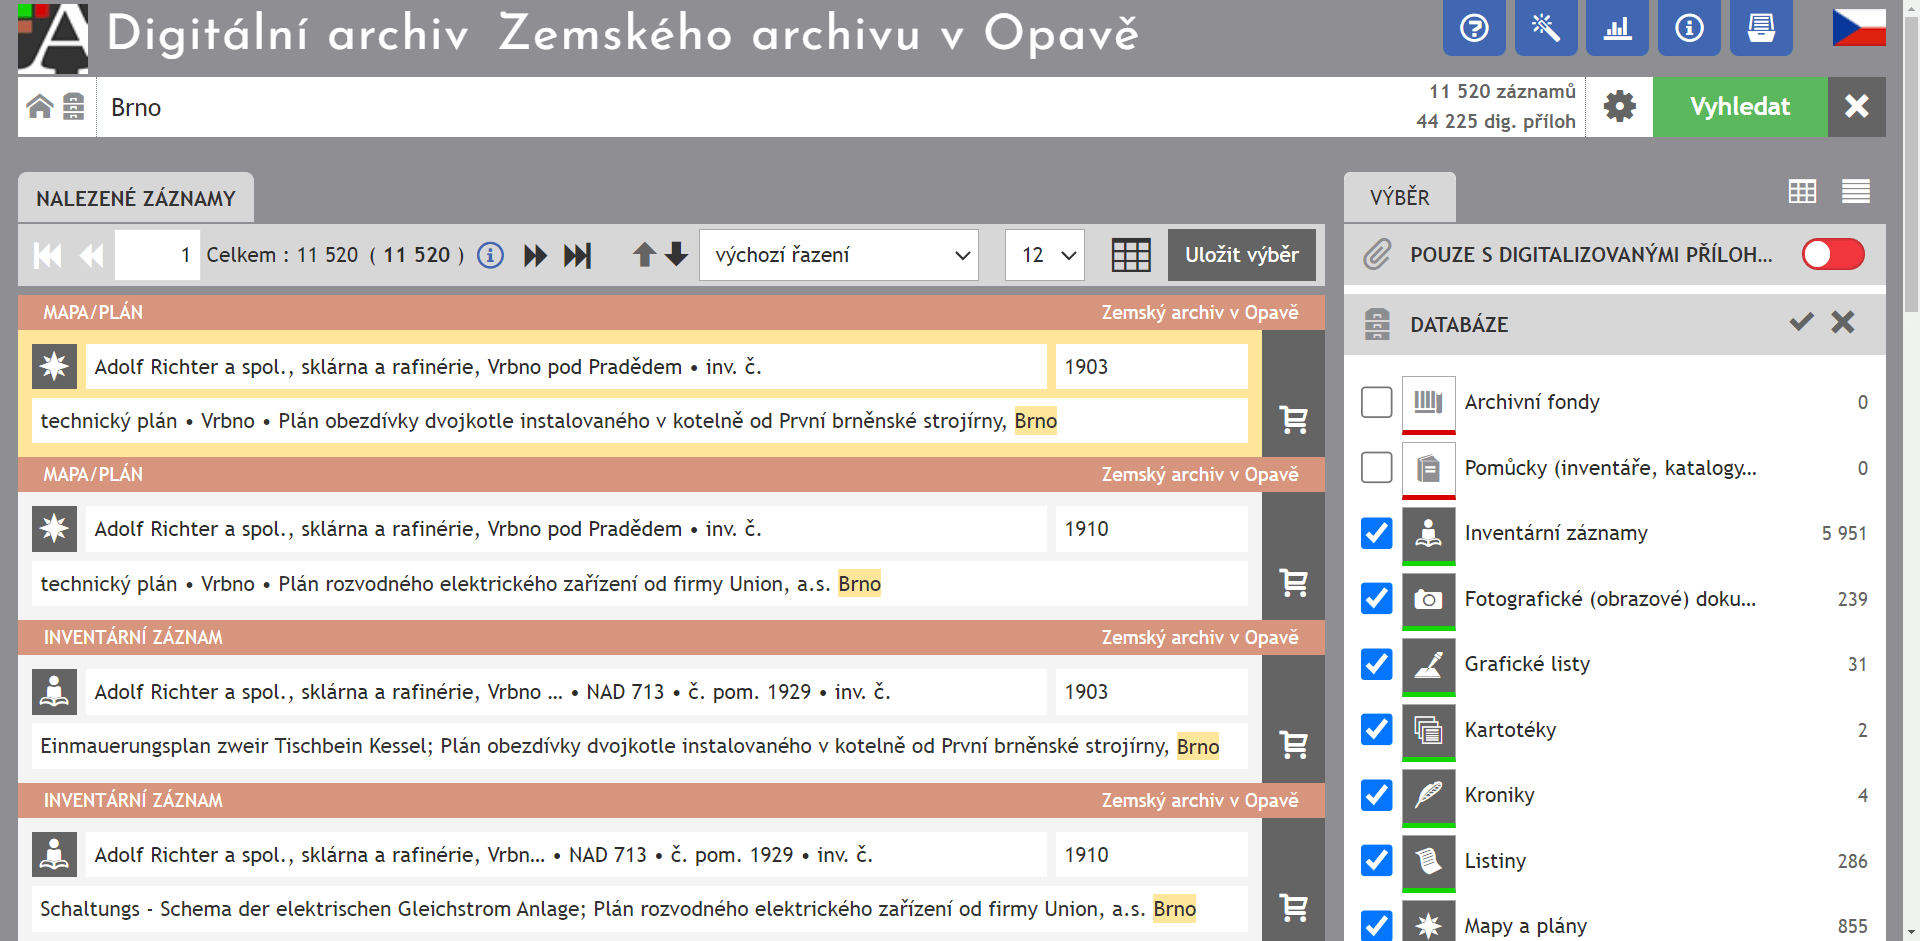
\includegraphics[scale=.2]{obrazky-figures/archives/zaOpava/vyhledani.png}
    \caption{Vyhledávání archiválií v~systému Zemského archivu v Opavě}
\end{figure}

\noindent
Nalezení SearchBean a~odkazu na soubory s příponou jspf napovídá, že se jedná nejen o~vzhledově podobné, ale i~o~aplikace postavené na stejném základu s~jistou mírou přizpůsobení. Aplikace Zemského archivu v Opavě běží na Apache Tomcat 4.1+. Obsahuje javascriptové knihovny jako například jQuery, less a~jistou míru vlastního javascript kódu. Obdobně jako Národní archiv používá knihovnu Zoomify pro efektivní zobrazování skenů archiválií. Dle mého názoru se jedná o~dost podobné aplikace, které sdílí své klady, ale i~zápory, které je zužují.

\begin{figure}[htbp]
\centering
    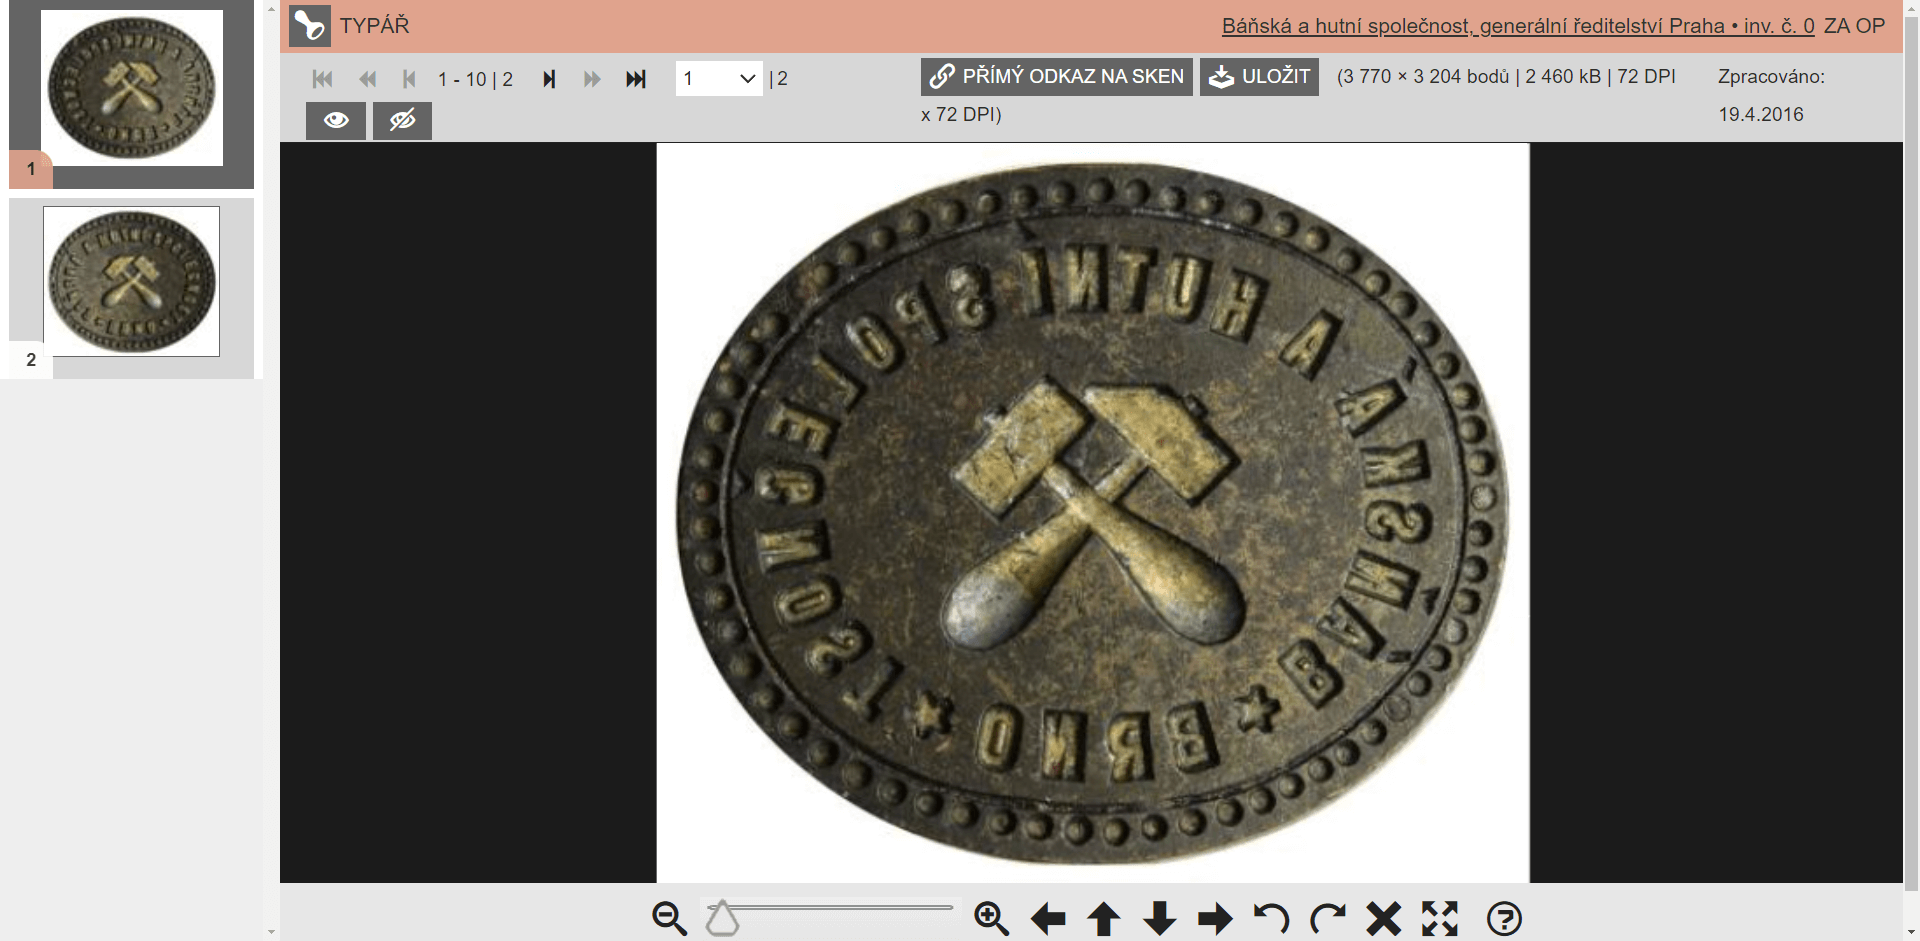
\includegraphics[scale=.2]{obrazky-figures/archives/zaOpava/prohlizec.png}
    \caption{Prohlížeč archiválií v~systému Zemského archivu v Opavě}
\end{figure}

\section{Státní oblastní archiv v~Třeboni}
Státní oblastní archiv v~Třeboni zpřístupňuje své materiály pomocí aplikace \href{https://digi.ceskearchivy.cz}{Digiarchiv}\footnote{https://digi.ceskearchivy.cz}. Rozložení i~vzhled aplikace je originální a~nepodobá se doposud porovnávaným systémům.V~kartě Hledání je možnost filtrovat jednotlivé archiválie podle typu archiválie, archivu i~datace. Dále umožňuje vyhledávání nejen pomocí inventárního čísla, ale i~plné textové vyhledávání podle klíčového slova.

\begin{figure}[htbp]
\centering
    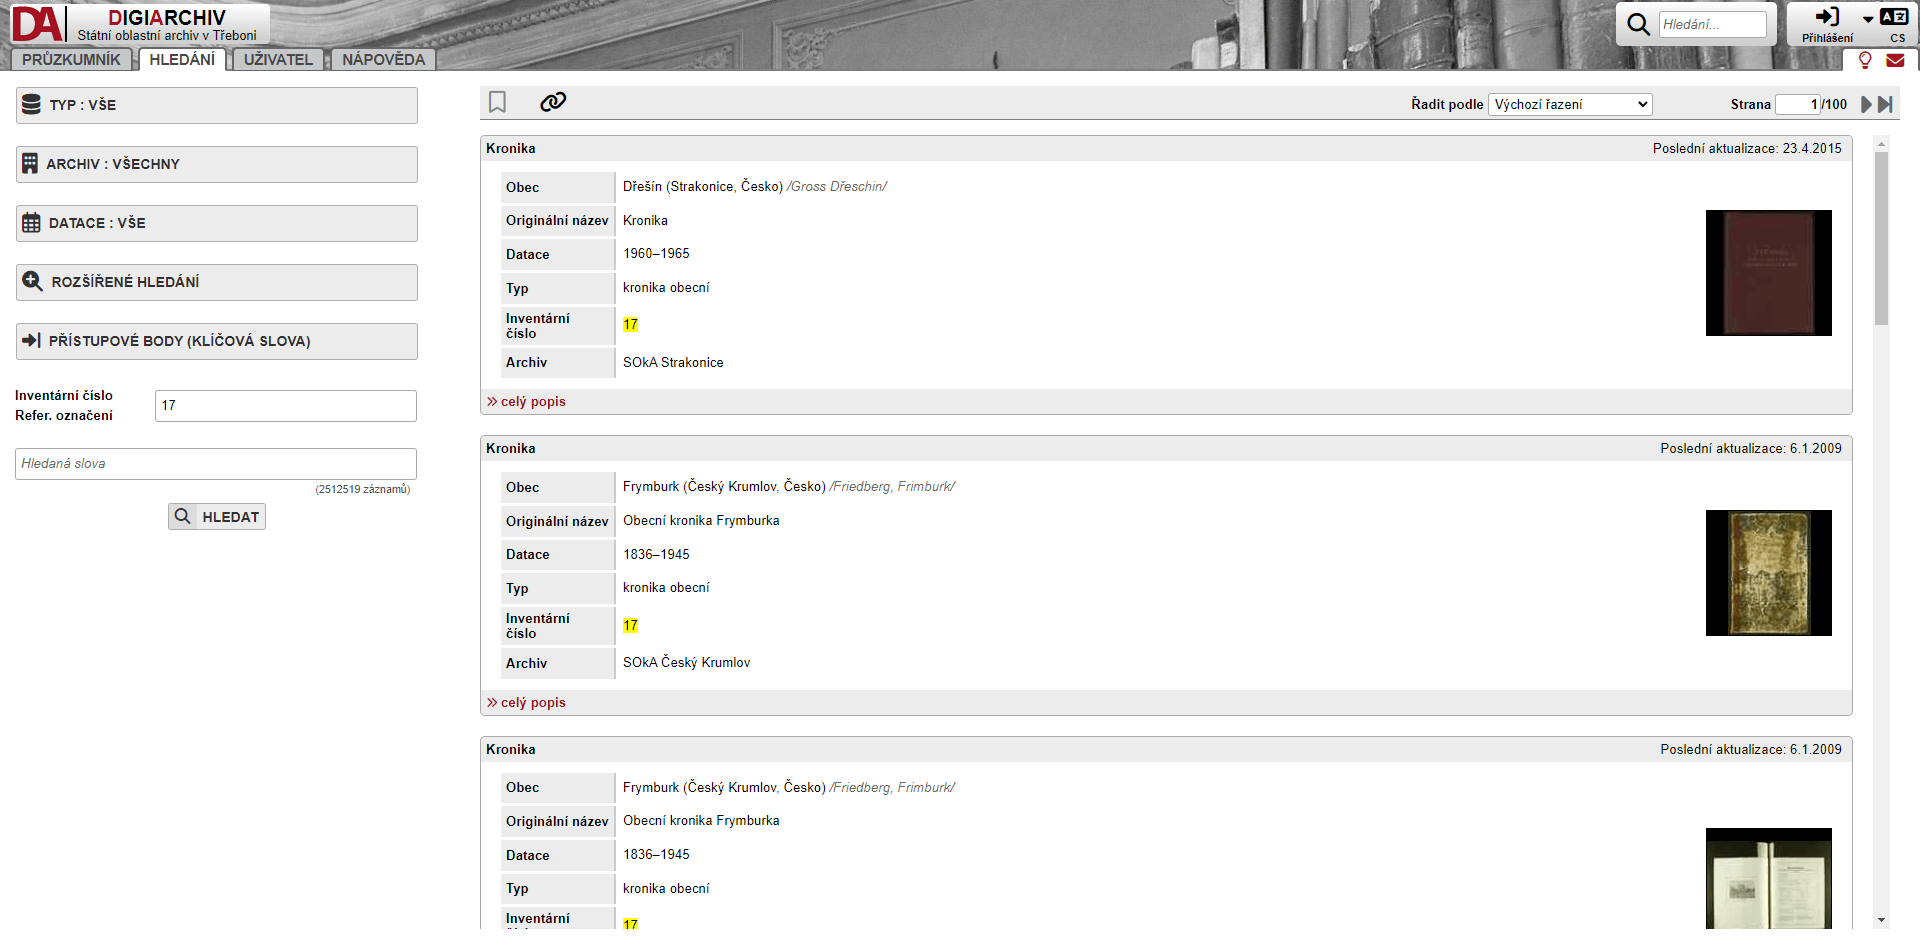
\includegraphics[scale=.2]{obrazky-figures/archives/soaTrebon/vyhledani.png}
    \caption{Vyhledávání archiválií v~systému SOA v~Třeboni}
\end{figure}
\noindent
Aplikace je hostována na Apache s PHP ve verzi 8.1.10. Z~javascriptových knihoven je zde využito Tipped a~jQuery. Samotná část webu, která je určena k~prohlížení archiválií, je zabalena v~iframu a~používá javascriptovou knihovnu ckeditor. Aplikace pro zobrazování skenů využívá dlaždicový formát, který je dostupný ze složky cgi-bin, což značí, že jsou dlaždice snímků generovány externím skriptem na webovém serveru. Pro kompletaci snímků v~prohlížeči se používá knihovna viewer-cs, ve které se vyskytuje klíčové slovo Zoomify a~IIIF, tudíž lze předpokládat, že právě tyto formáty jsou v rámci systému použity.

\begin{figure}[htbp]
\centering
    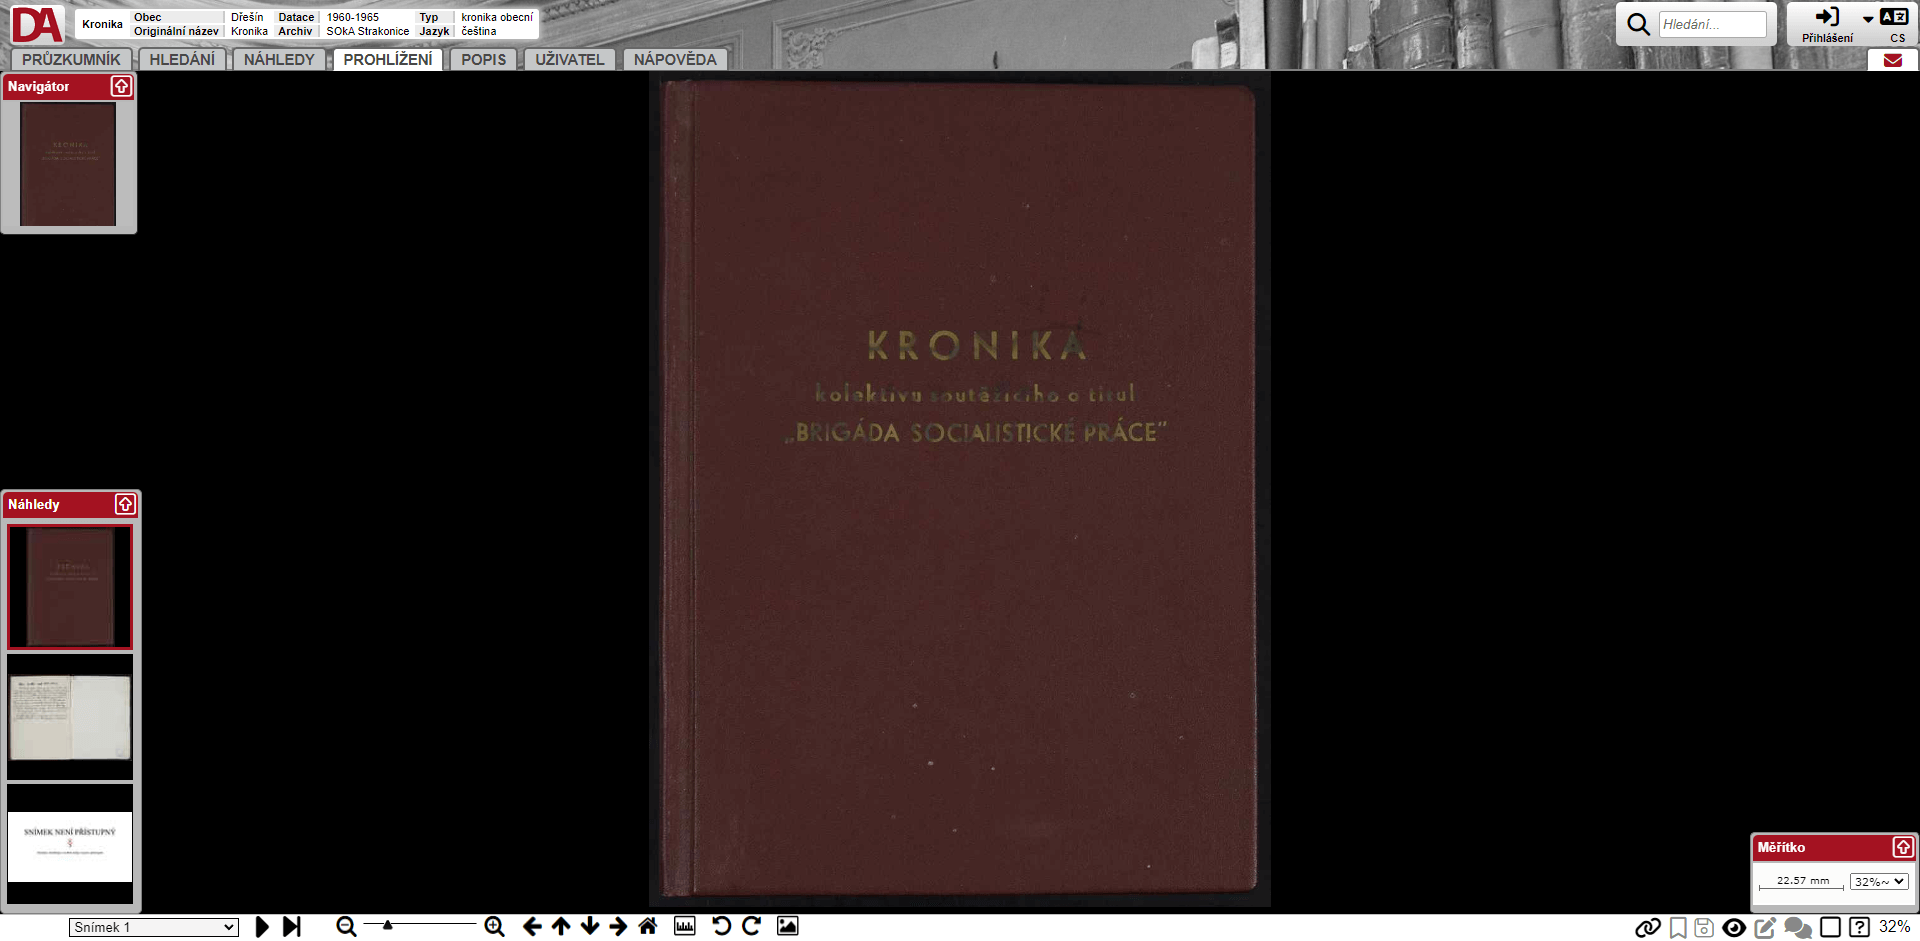
\includegraphics[scale=.2]{obrazky-figures/archives/soaTrebon/prohlizec.png}
    \caption{Prohlížeč archiválií v~systému SOA v~Třeboni}
\end{figure}

\noindent
Samotný prohlížeč nechává dostatek prostoru pro zobrazení skenu archiválie. Na pravé straně obsahuje náhledy dalších skenů a~v~dolní části je umístěno bohaté nastavení včetně filtrů, jež lze na snímek aplikovat. Hlavní nevýhodou prohlížeče je přechod mezi archiváliemi, který zapříčiní přenačtení celého webu a~samotná operace trvá okolo jedné vteřiny. Tato odezva je negativně citelná v~případě, kdy badatel chce rychle projít celou archiválii nebo~hledá konkrétní informaci.

\section{Státní oblastní archiv v~Litoměřicích}
Státní oblastní archiv v~Litoměřicích poskytuje aplikaci \href{http://vademecum.soalitomerice.cz/vademecum}{Vademecum}\footnote{http://vademecum.soalitomerice.cz/vademecum}. Jak již název napovídá, jedná se o totožnou aplikaci, jako má Národní archiv a~Zemský archiv v~Opavě, přičemž se více podobá digitálnímu archivu z~Opavy. Aplikace běží na Javě, využívá podpůrné javascriptové knihovny a  formát Zoomify pro zobrazení snímků.
\begin{figure}[htbp]
\centering
    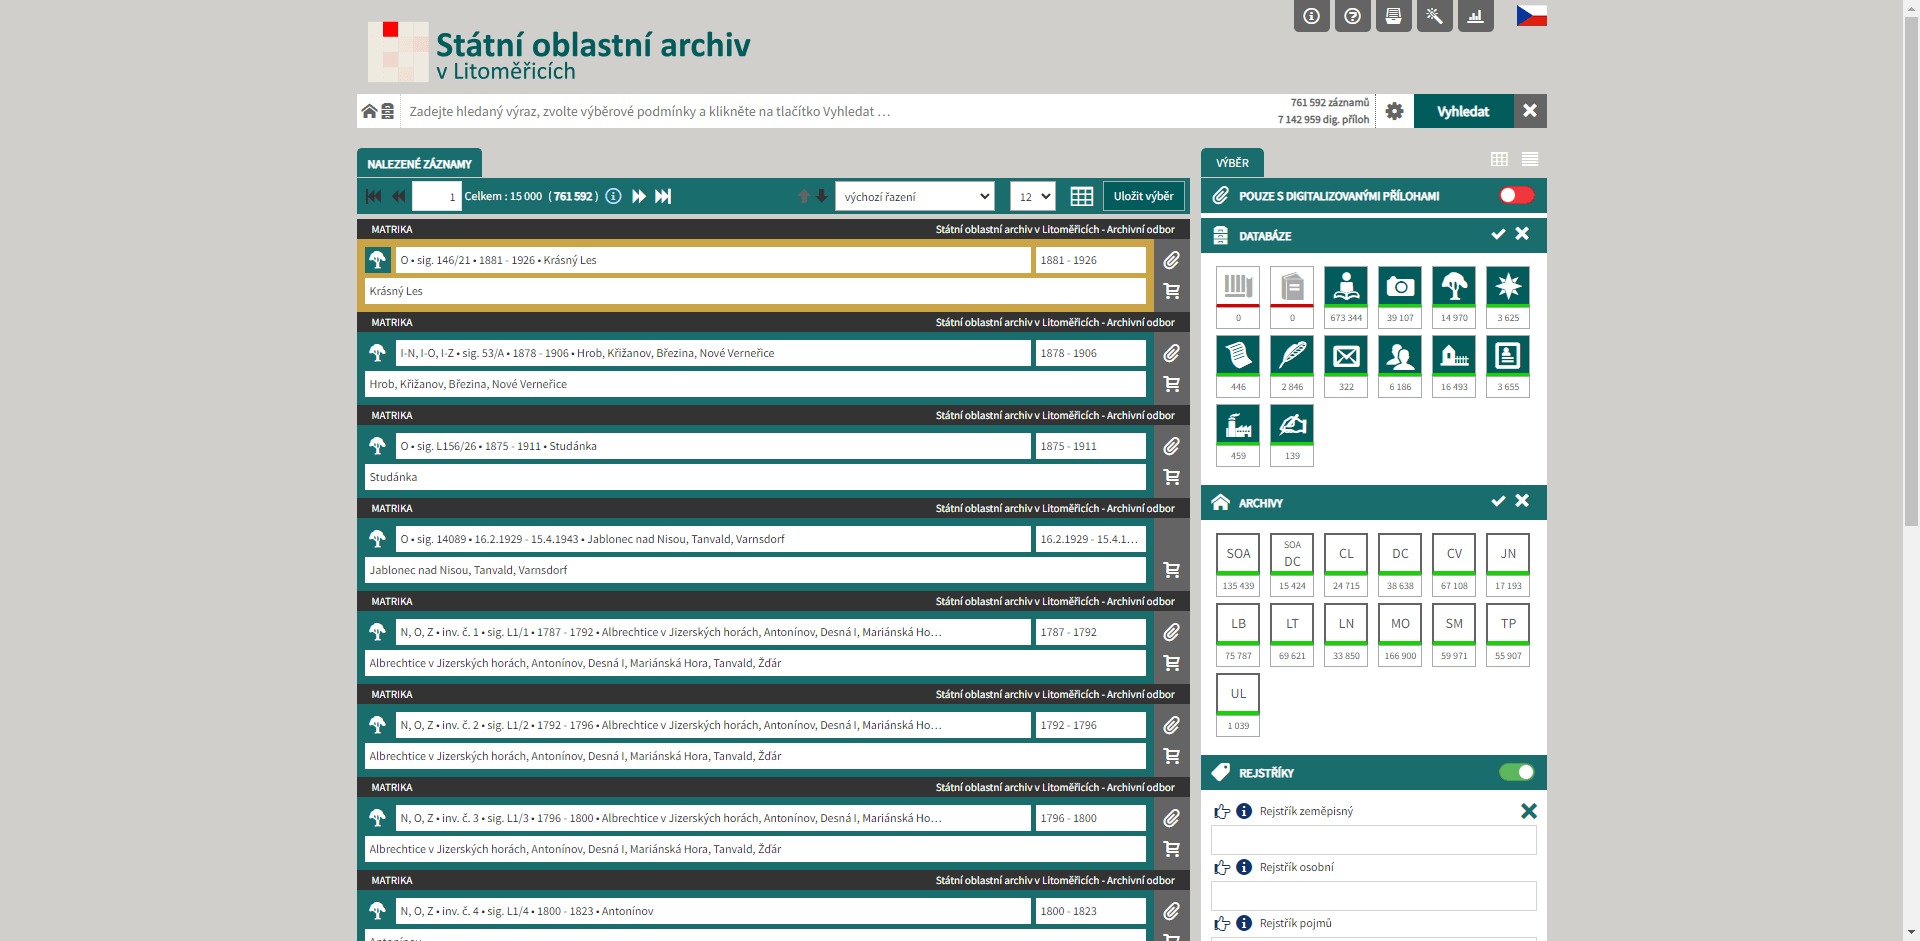
\includegraphics[scale=.2]{obrazky-figures/archives/soaLitomerice/vyhledani.png}
    \caption{Vyhledávání archiválií v~systému SOA v~Litoměřicích}
\end{figure}

\newpage
\section{Státní oblastní archiv v~Plzni}
Státní oblastní archiv v~Plzni poskytuje své archiválie prostřednictvím \href{https://www.portafontium.eu}{Porta Fontium}\footnote{https://www.portafontium.eu}. Systém nabízí rozdělení jednotlivých záznamů do hierarchické struktury podle původce a~oblasti. Toto dělení je podobné systému \href{http://radegast.fit.vutbr.cz/}{Demos}\footnote{http://radegast.fit.vutbr.cz}. 
Dále zde lze vyhledávat pomocí místa, textu a~roku. Aplikace umožňuje procházet všechny archiválie nebo filtrovat konkrétní typ archiválií.

\begin{figure}[htbp]
\centering
    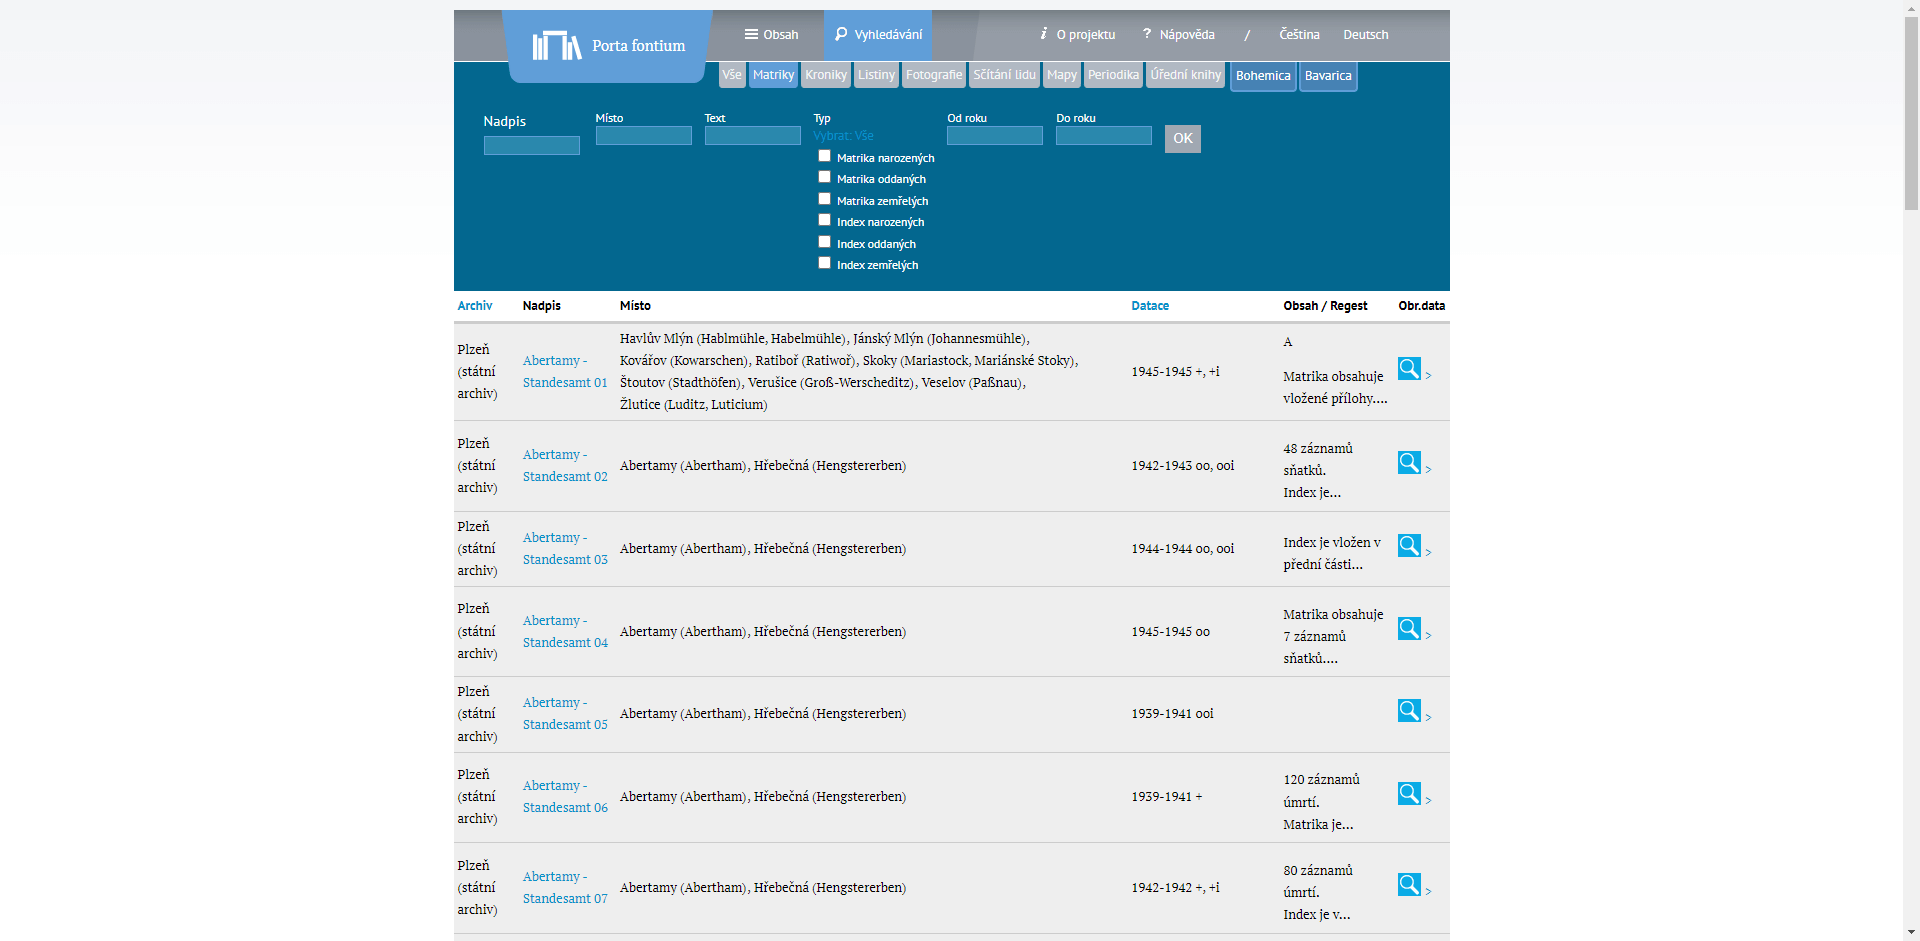
\includegraphics[scale=.2]{obrazky-figures/archives/soaPlzen/vyhledani.png}
    \caption{Vyhledávání archiválií v~systému SOA v~Plzni}
\end{figure}

\noindent
Analýzou komunikace bylo zjištěno, že běží na CMS Drupal 7, který je napsaný v~jazyce PHP. Snímky jsou uloženy ve složce fcgi-bin, což nám obdobně jako u~Státního oblastního archivu v~Třeboni značí, že jsou generovány externím skriptem. Pro dlaždicový formát obrázků zde byl zvolen formát Deepzoom. Z~javascriptových knihoven jsou použity Drupal.JS a~jQuery. 
\newpara
Prohlížeč snímků archiválií je dobře rozložen, obsahuje standardní navigaci nad snímkem archiválie i~náhled dalších stran v~levém panelu. Z~mého pohledu plně nevyužívá plochu pro snímek, která je na stránce k~dispozici. Tento nedostatek je negován kvalitním režimem celé obrazovky, který kromě subtilního horního menu zobrazuje archiválii na celé obrazovce. Rychlost načítání je dostatečná a přechod mezi snímky je plynulý. Systém postrádá možnost úpravy jasu a~kontrastu snímku společně s libovolnou rotací snímku.

\begin{figure}[htbp]
\centering
    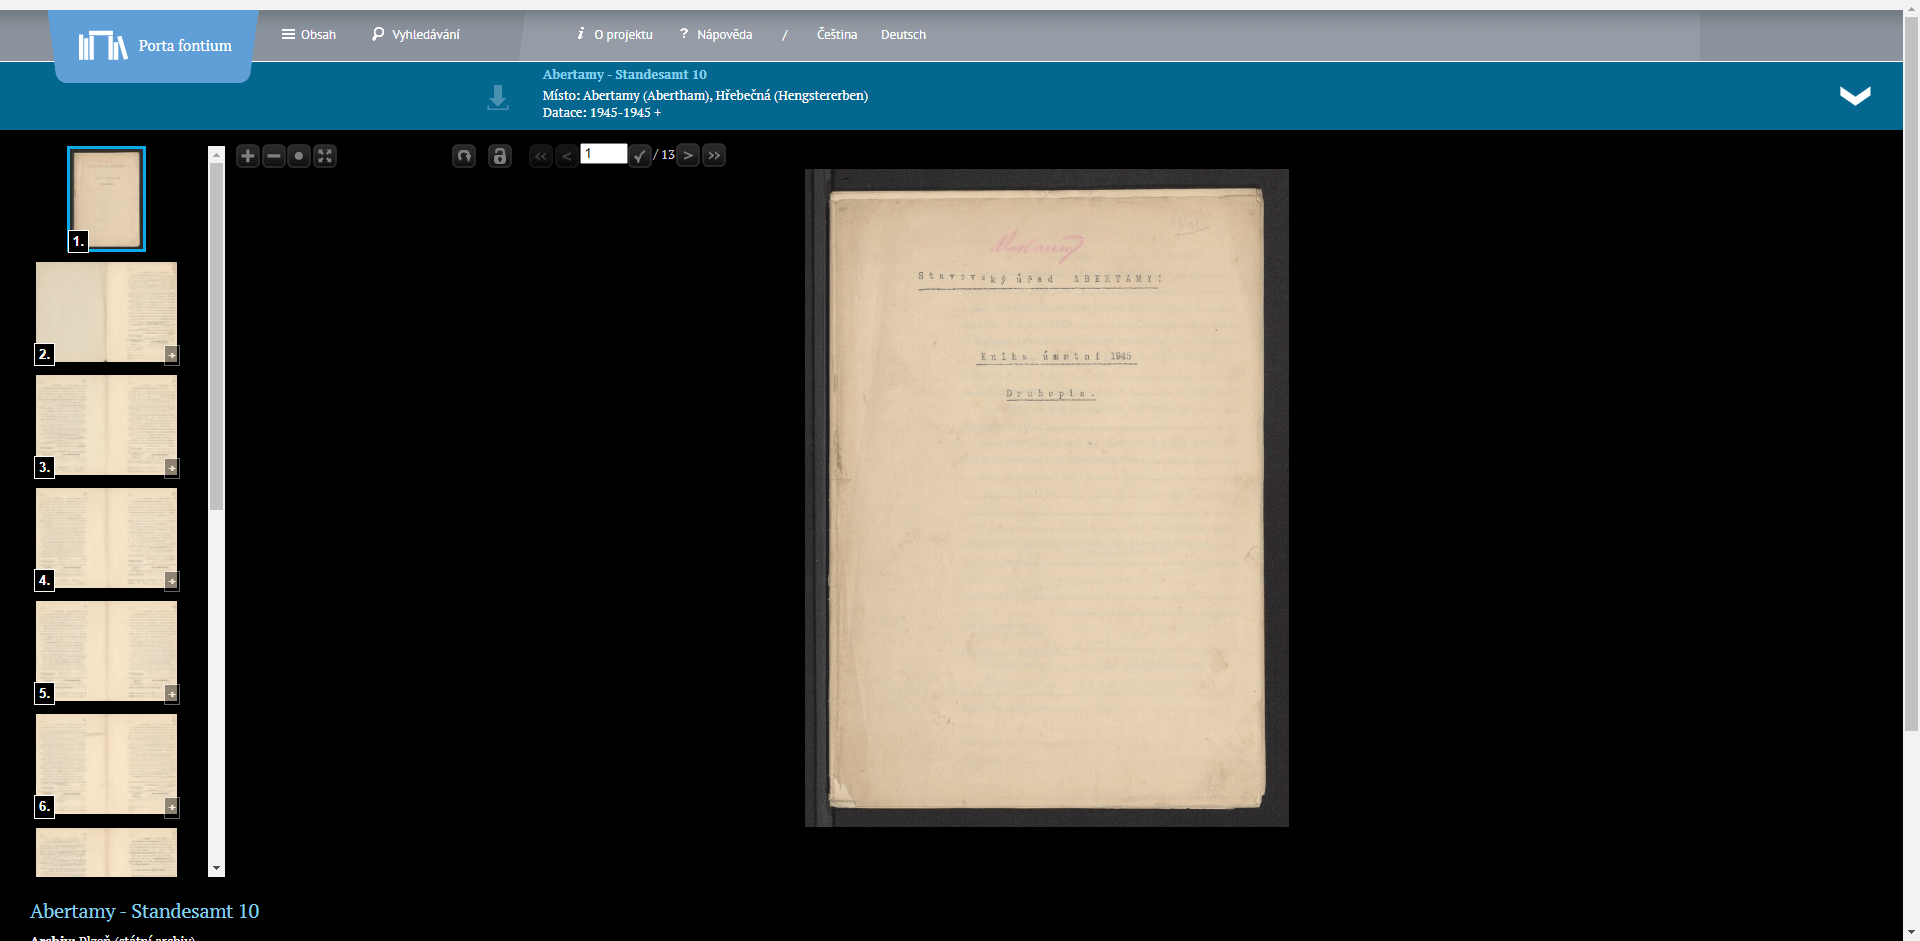
\includegraphics[scale=.2]{obrazky-figures/archives/soaPlzen/prohlizec.png}
    \caption{Prohlížeč archiválií v~systému SOA v~Plzni}
\end{figure}


\section{Státní oblastní archiv v~Hradci Králové}
Státní oblastní archiv v~Hradci Králové poskytuje své materiály skrze aplikaci \href{https://aron.vychodoceskearchivy.cz}{Archivy Online}\footnote{https://aron.vychodoceskearchivy.cz}. Aplikace disponuje moderním uživatelským rozhraním a bohatým nastavením pro filtrování archivních záznamů.

\begin{figure}[htbp]
\centering
    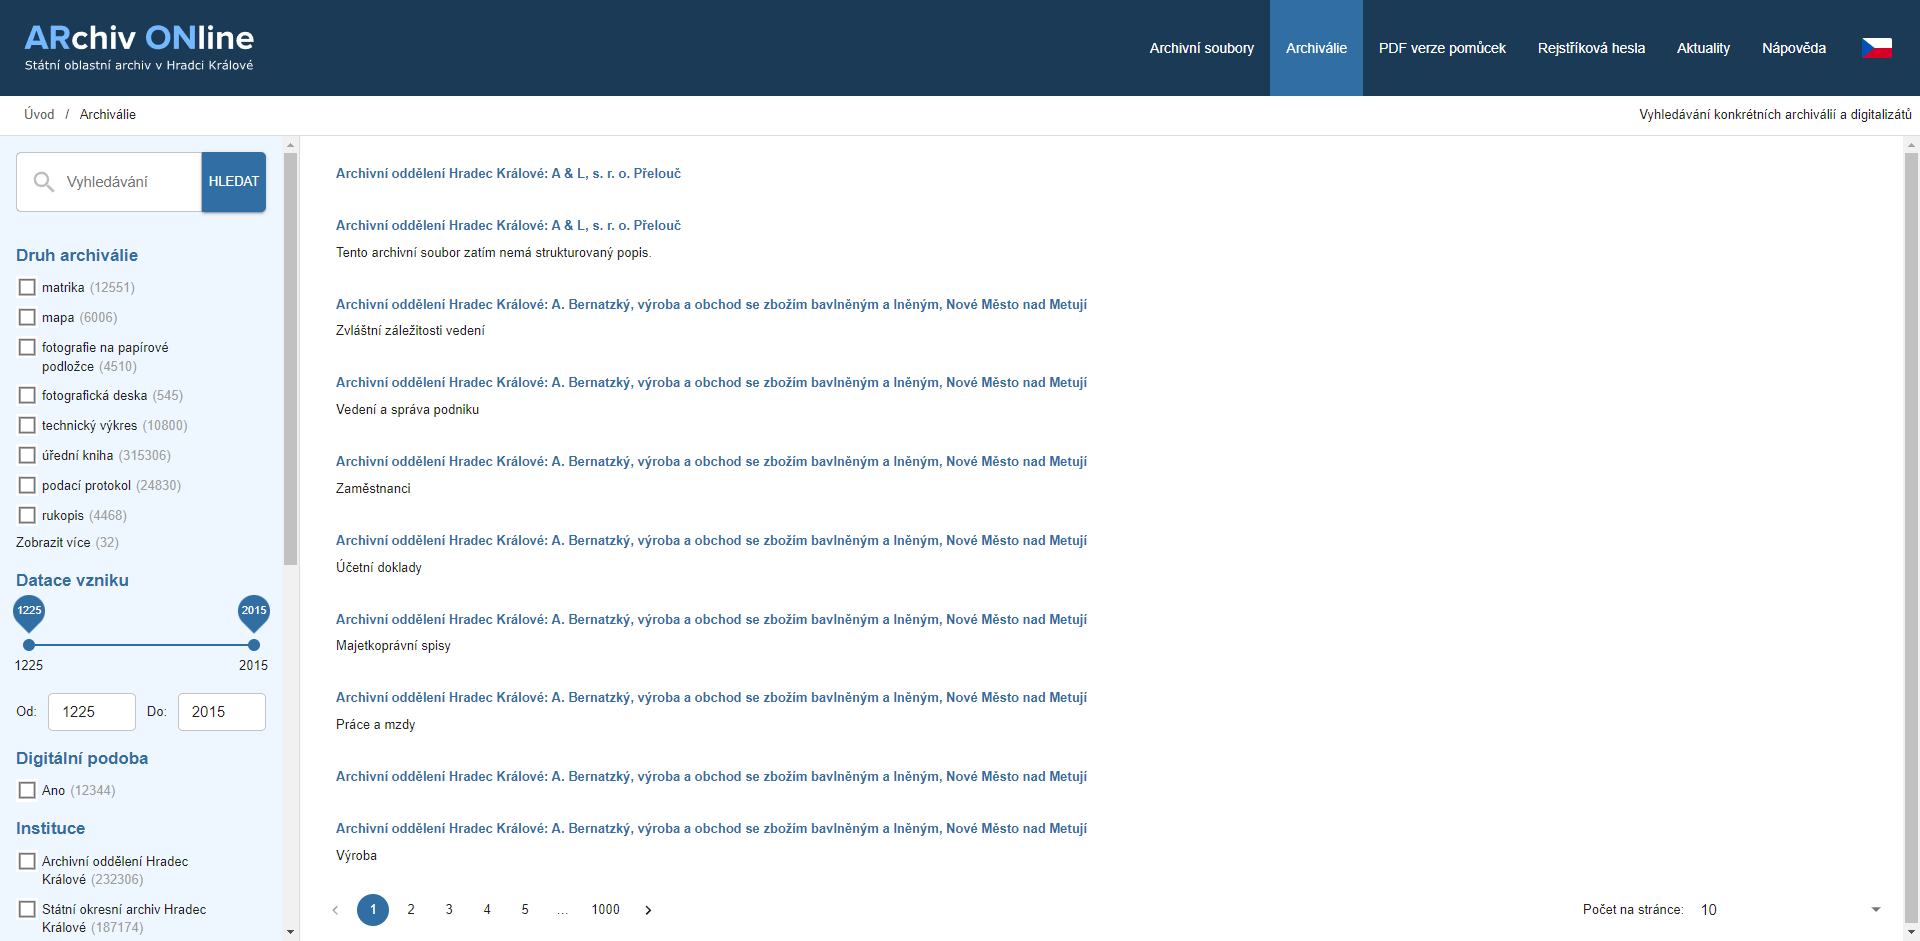
\includegraphics[scale=.2]{obrazky-figures/archives/soaHradecKralove/vyhledani.png}
    \caption{Vyhledávání archiválií v~systému SOA v~Hradci Králové}
\end{figure}
\newpage
\noindent
ARON je první aplikace v~tomto seznamu, jež využívá separátní aplikaci pro zobrazování klientské části, která komunikuje s~API. Klientská část aplikace je napsána v~reaktivním javascriptovém aplikačním rámci React.JS ve verzi 16. Po zaslání separátního dotazu na API byla obdržena upravená odpověď 404. Z~odpovědi se dá usoudit, že serverová část aplikace běží na Javě, vzhledem k~moderní volbě technologie pro frontend se dá očekávat aplikační rámec nad Javou jako například Spring. Pro zobrazování snímků archiválií je zde využita javascriptová knihovna \href{https://openseadragon.github.io}{OpenSeaDragon}\footnote{https://openseadragon.github.io} a jednotlivé snímky jsou uloženy v~dlaždicovém formátu Deepzoom.
\newpara
Prohlížeč snímků archiválií obsahuje mnoho meta informací, takže nezbývá dostatek prostoru pro samotný snímek. Malou plochu pro snímek na detailu archiválie kompenzuje režim celé obrazovky, kde se již dá s daným snímkem plnohodnotně pracovat. Aplikace umožňuje daný snímek stáhnout ve~vysoké kvalitě a~obsahuje základní manipulační nástroje, mezi něž například patří rotace obrazu. Zde jsem bohužel narazil na problém, kdy snímek lze otáčet pouze po 90° a~daná archiválie byla otočena o 45°, což znemožňovalo natočení řádků do vodorovné polohy. Aplikace dále podporuje klávesové zkratky a~jako celek funguje velmi obstojně.

\begin{figure}[htbp]
\centering
    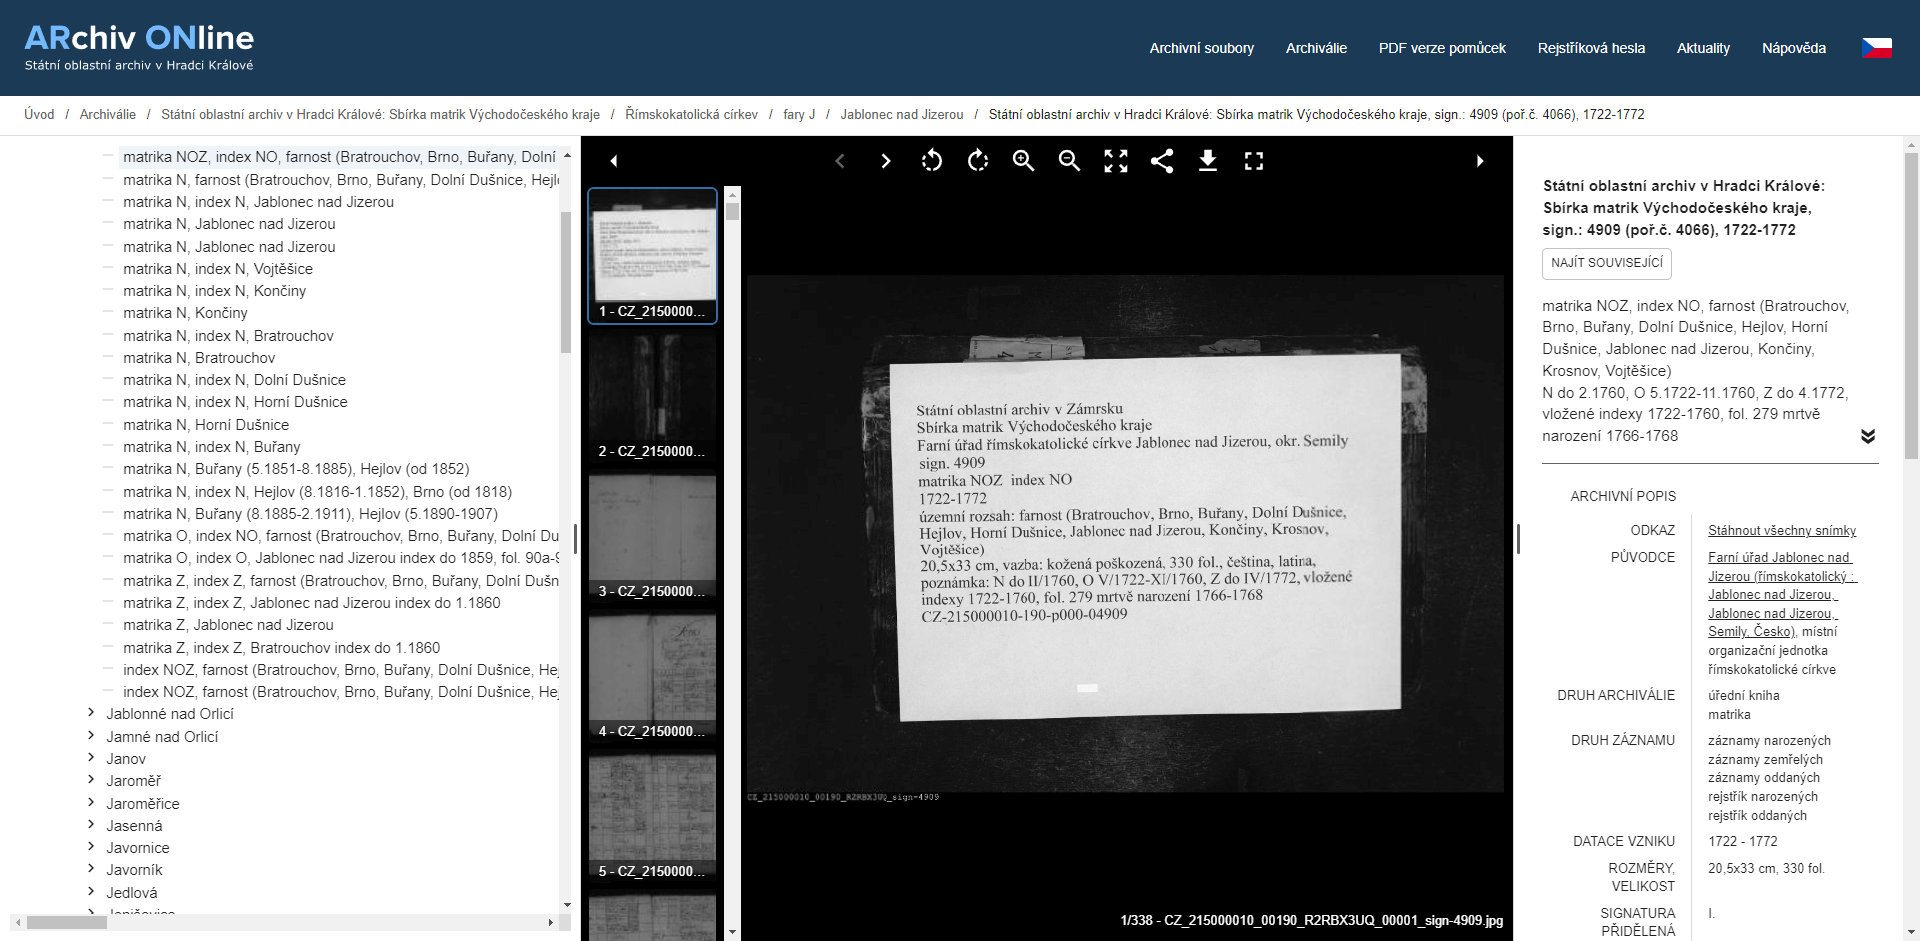
\includegraphics[scale=.2]{obrazky-figures/archives/soaHradecKralove/prohlizec.png}
    \caption{Prohlížeč archiválií v~systému SOA v~Hradci Králové}
\end{figure}

\newpage
\section{Státní oblastní archiv v~Praze}
Státní oblastní archiv v~Praze poskytuje svoje archiválie skrze \href{https://ebadatelna.soapraha.cz}{eBadatelnu}\footnote{https://ebadatelna.soapraha.cz}. Matriky aplikace zvládá vyhledávat pomocí lokality, názvu a~původce. Dále je možné specifikovat časový rozsah a jednotlivé výsledky jsou zobrazeny pomocí standardní tabulky.

\begin{figure}[htbp]
\centering
    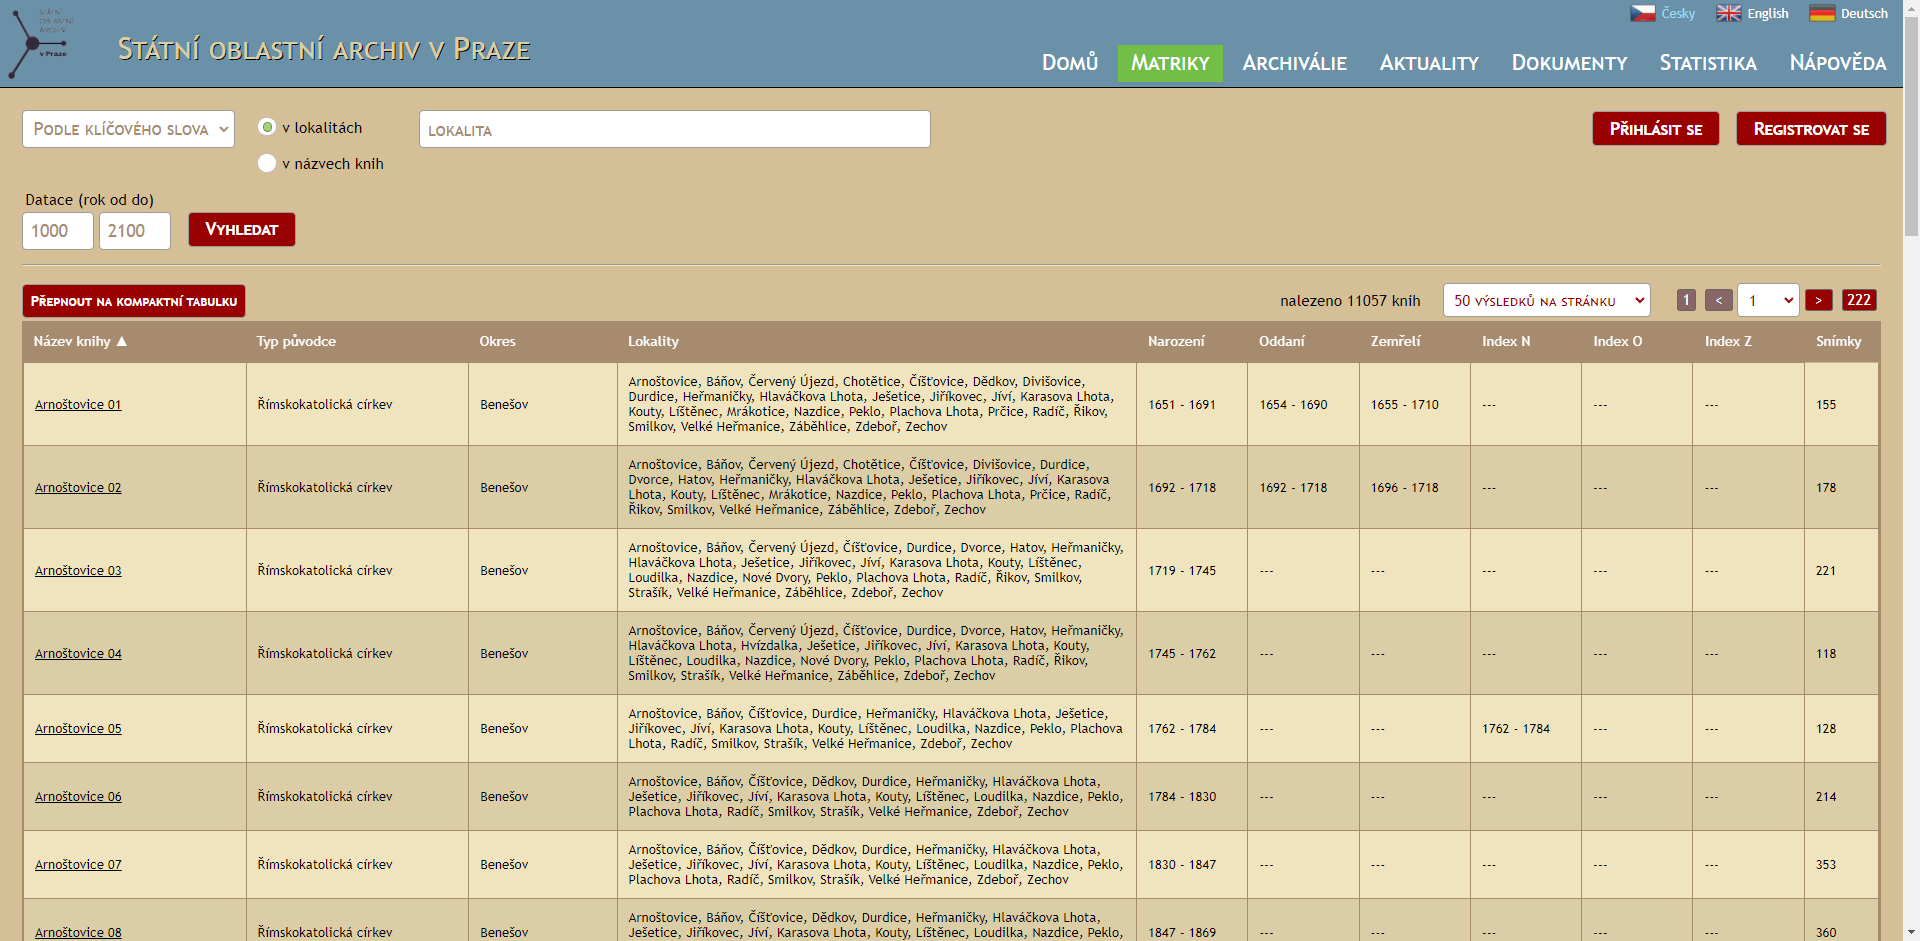
\includegraphics[scale=.2]{obrazky-figures/archives/soaPraha/vyhledani.png}
    \caption{Vyhledávač archiválií v~systému SOA v~Praze}
\end{figure}

\newpage
\noindent
Na základě analýzy bylo zjištěno, že aplikace využívá webový aplikační rámec Apache Wicket, který je napsaný v~Javě. Z~JavaScriptových knihoven využívá AJAX pro asynchronní nahrávání obsahu a~jQuery.
\newpara
Prohlížeč snímků archiválií nabízí možnost rotace a~navigace mezi snímky. Možnost náhledu dalších snímků zde chybí. Při změně snímku probíhá přenačtení celé aplikace a snímky jsou stahovány rovnou v plné kvalitě. Tato kombinace tvoří velmi pomalé rozhraní a~změna snímku zde trvá v~řádu několika vteřin. Libovolná manipulace s archiválií jako například přiblížení nebo pohyb není plynulá, což snižuje uživatelskou přívětivost pro badatele při práci s tímto systémem.

\begin{figure}[htbp]
\centering
    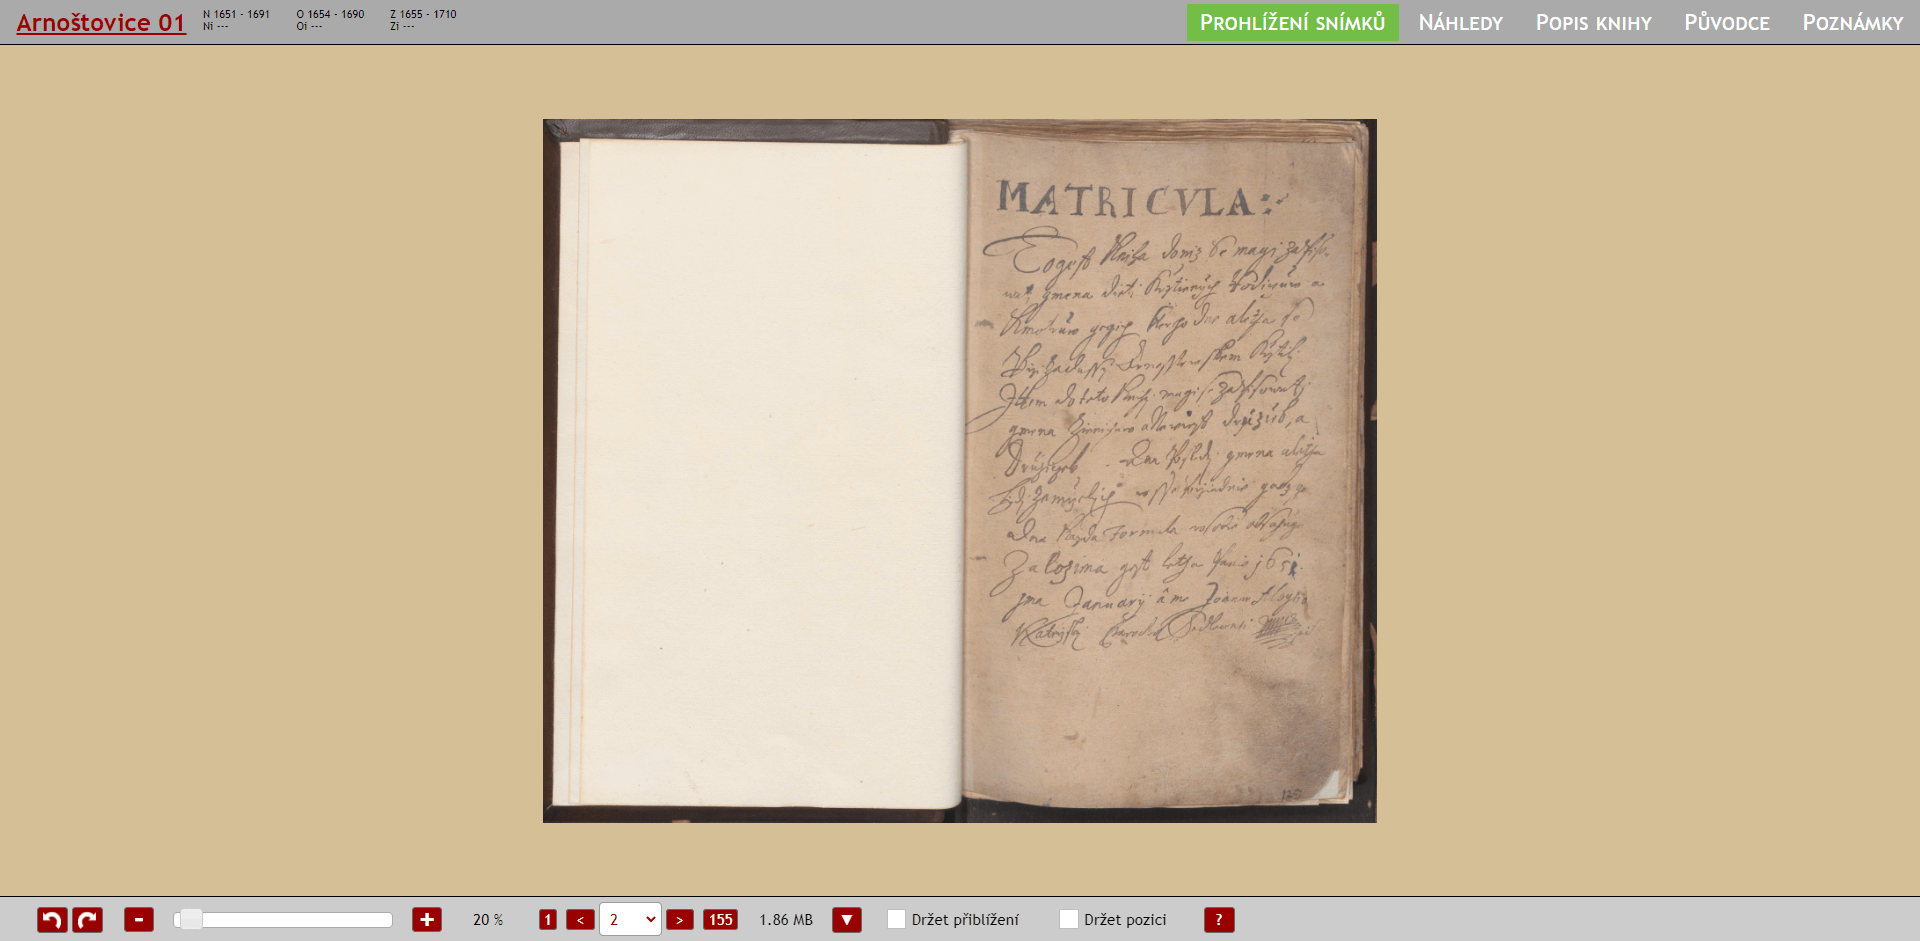
\includegraphics[scale=.2]{obrazky-figures/archives/soaPraha/prohlizec.png}
    \caption{Prohlížeč archiválií v~systému SOA v~Praze}
\end{figure}

\section{Digitalizace evropských archivů}
Digitalizace evropských archivů poskytuje aplikaci \href{https://www.monasterium.net/mom/fonds}{Monasterium}\footnote{https://www.monasterium.net/mom/fonds} zpřístupňující archiválie z~více států včetně České republiky. Aplikace neobsahuje pokročilé vyhledávání a záznamy jsou organizovány pouze podle státu, města a~fondu. 

\begin{figure}[htbp]
\centering
    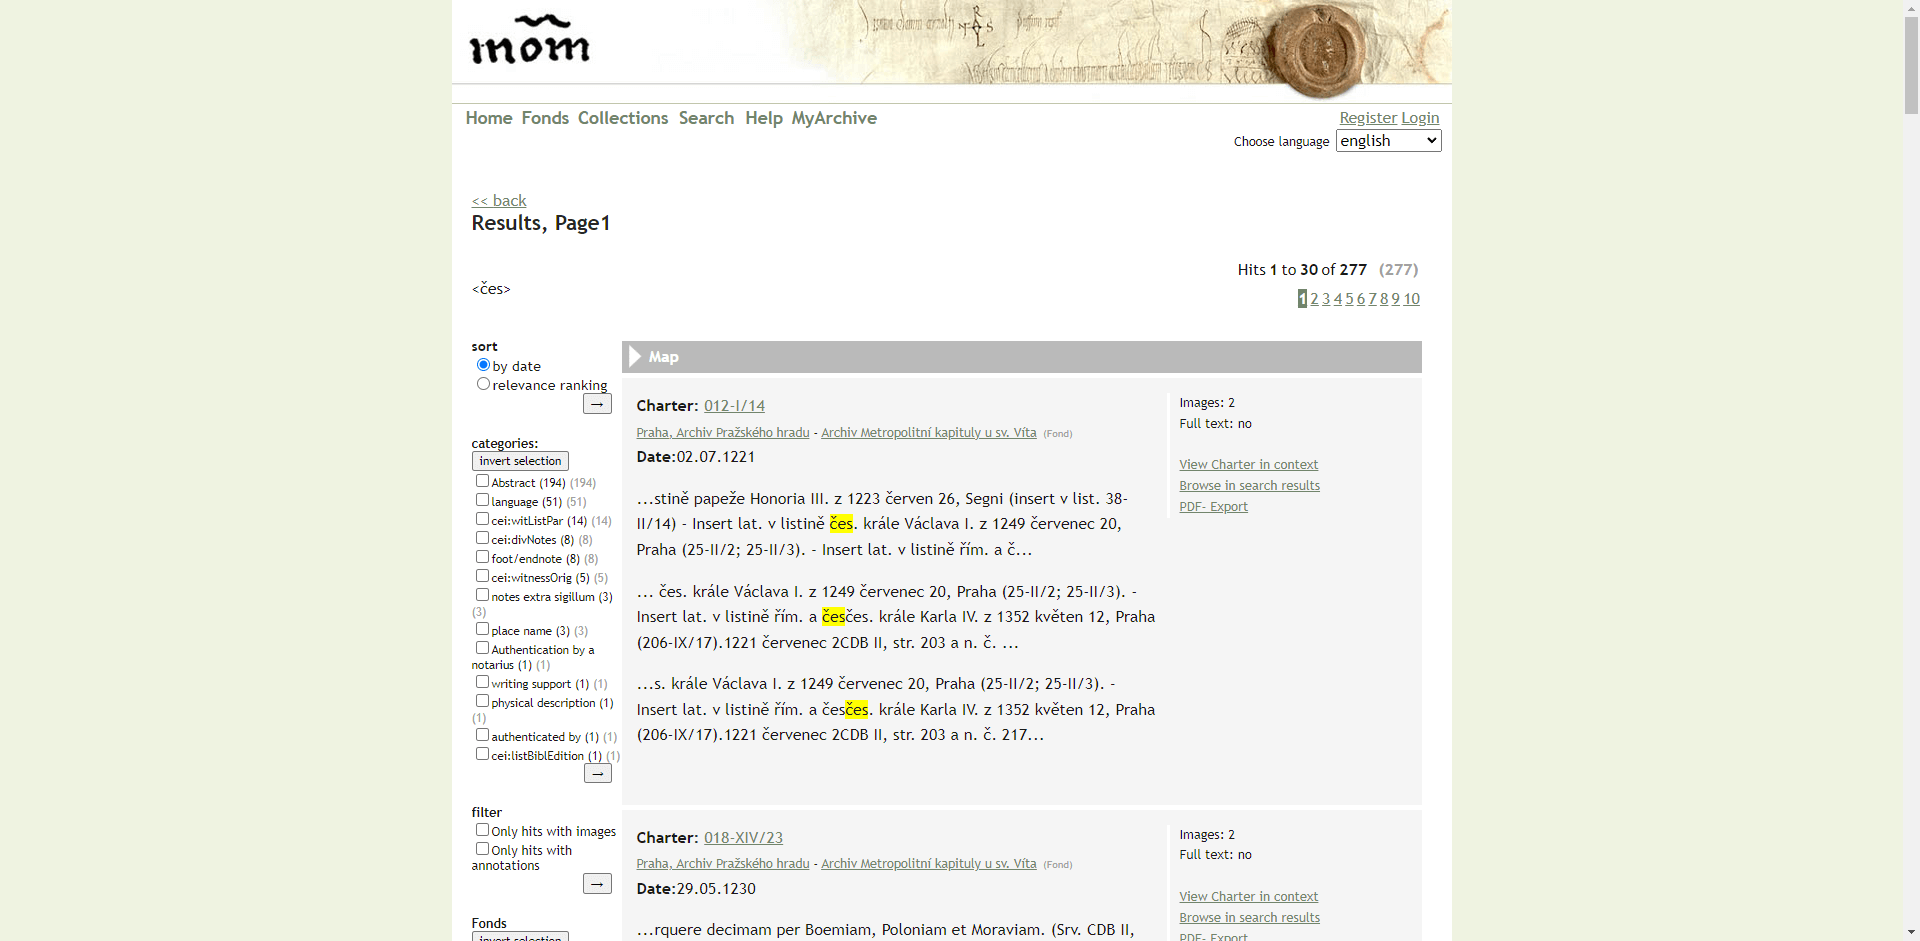
\includegraphics[scale=.2]{obrazky-figures/archives/mom/vyhledani.png}
    \caption{Vyhledávač archiválií v~systému Monasterium}
\end{figure}

\newpage
\noindent
Aplikace je napsána v~Javě a~běží v~kontejneru Jetty ve verzi 9.4.14. Z~JavaScriptových knihoven využívá pouze jQuery a~Leaflet pro zobrazení map.
\newpara
Prohlížeč archiválií zde disponuje omezenou sadou funkcí. Kromě navigace mezi stránkami neumožňuje upravit žádné nastavení, neposkytuje režim celé obrazovky a~pohyb po archiválii zde nefunguje pomocí táhnutí archiválie, ale pomocí vertikálního a~horizontálního scroll baru. Jediná možnost interakce se snímkem je pomocí scroll barů a~jednoho slideru pro nastavení přiblížení. Snímky nepoužívají žádný dlaždicový systém a~jsou přednačítány dopředu pro celou archiválii, což ze začátku prohlížení archiválie způsobuje prodlevu. Celková plocha pro prohlížení snímku je velmi malá a~při kliknutí na daný snímek se pouze zobrazí v~prohlížeči jako zdroj.

\begin{figure}[htbp]
\centering
    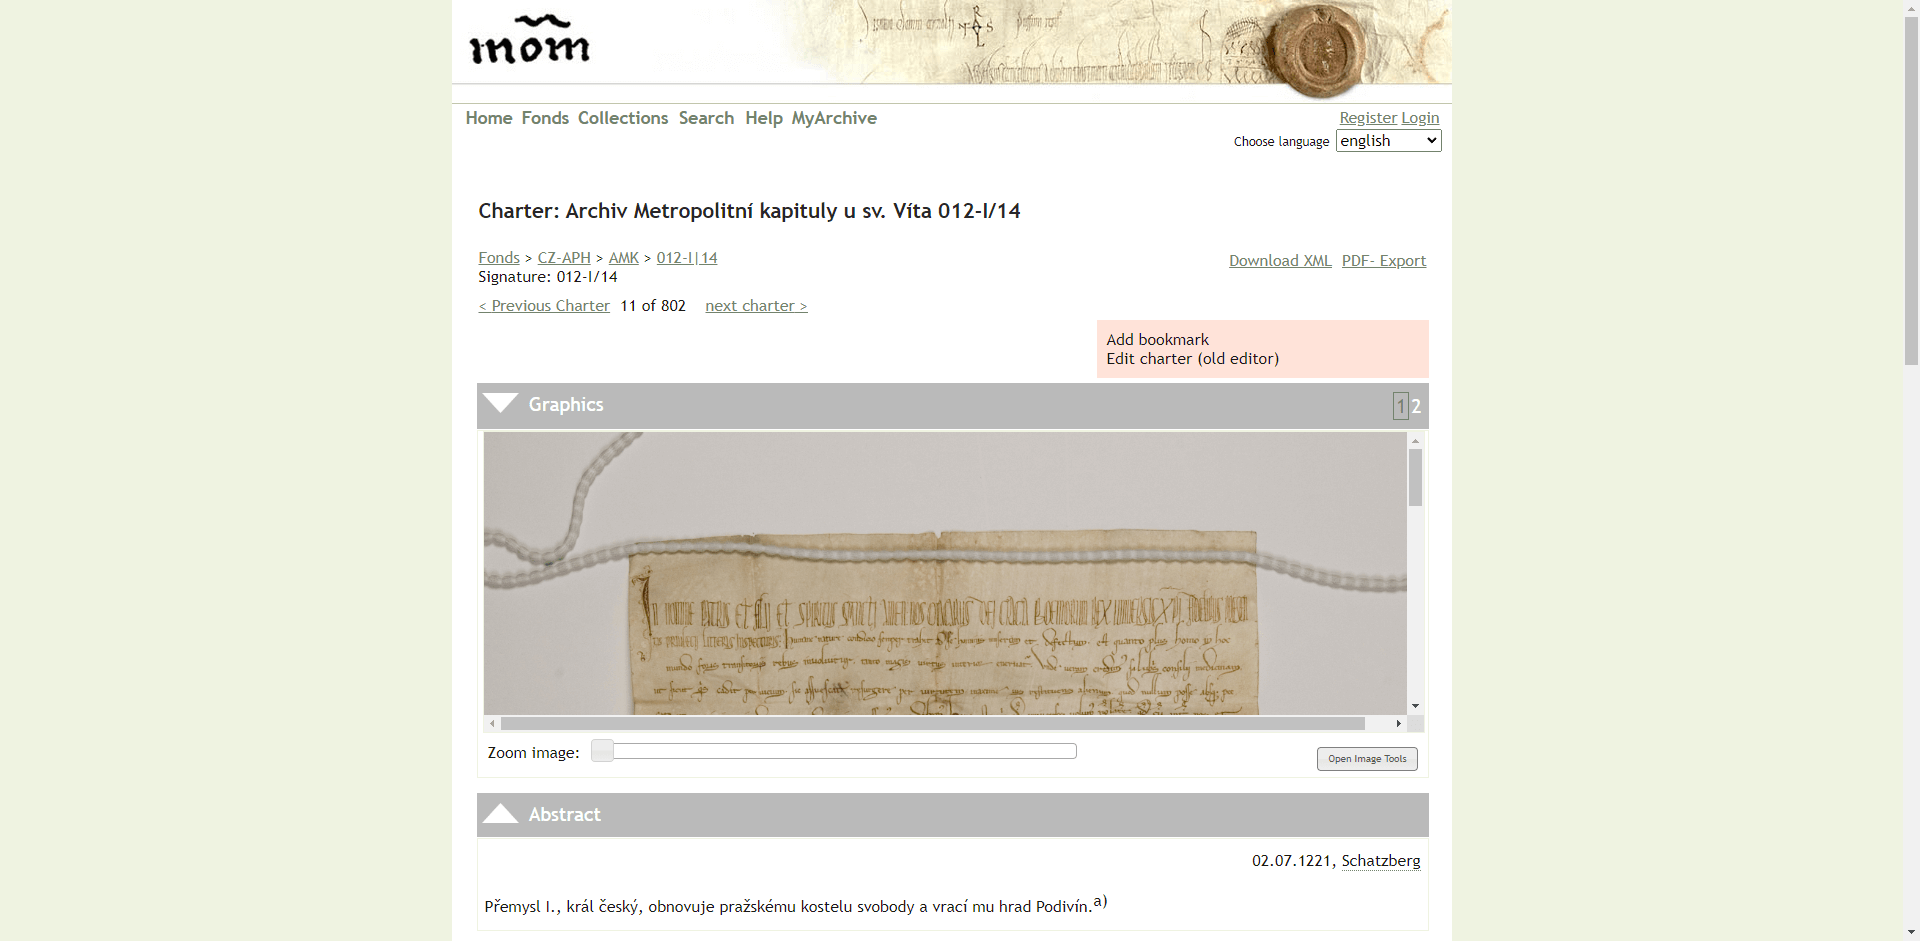
\includegraphics[scale=.2]{obrazky-figures/archives/mom/prohlizec.png}
    \caption{Prohlížeč archiválií v~systému Monasterium}
\end{figure}

\newpage
\section{Matricula online}
Dalším zástupcem mezinárodního prohlížeče matrik je \href{https://data.matricula-online.eu}{Matricula}\footnote{https://data.matricula-online.eu}. Aplikace umožňuje vyhledávat pomocí místa a~časového rozsahu. Dále je zde možné klasické prohledávání podle státu a~oblasti. Při volbě místa je aktualizována mapa, která zobrazuje místa, odkud archiválie pochází. Zobrazení matrik je provedeno standardní tabulkou s~možností filtrování druhu matriky a~časového období.

\begin{figure}[htbp]
\centering
    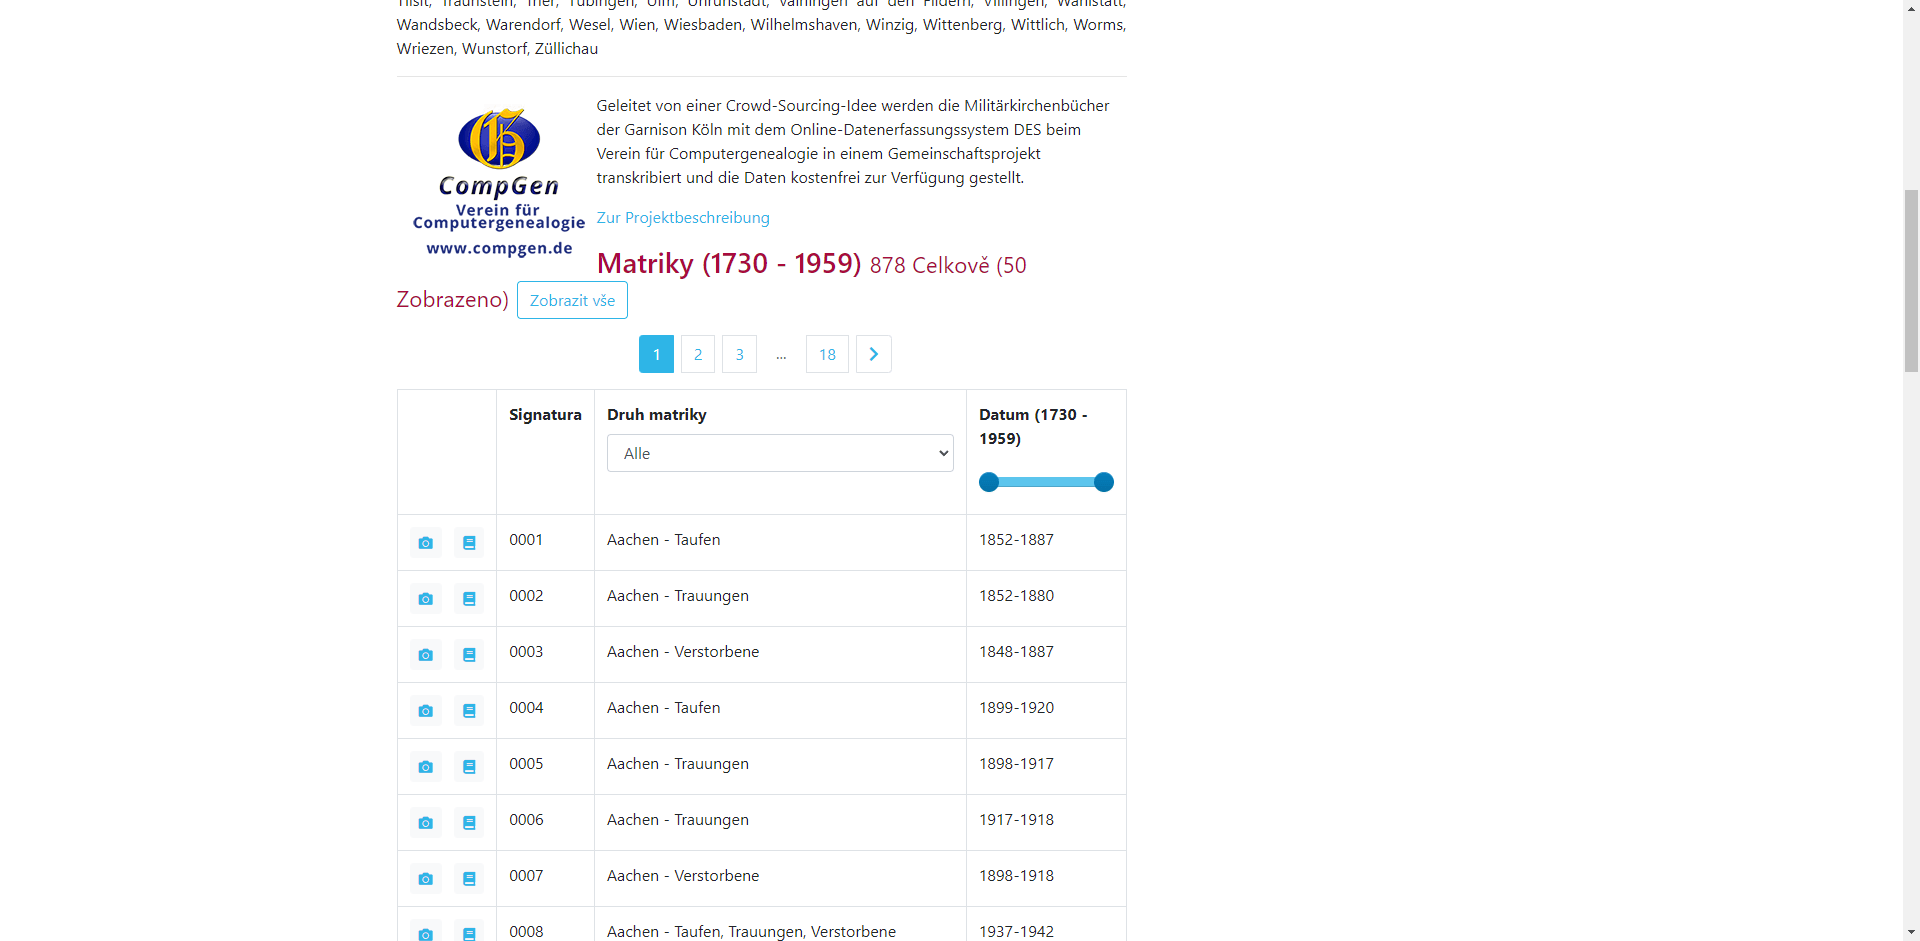
\includegraphics[scale=.2]{obrazky-figures/archives/matricula/vyhledani.png}
    \caption{Vyhledávač archiválií v~systému Matricula}
\end{figure}

\noindent
Aplikace je hostována na Apache 2.4.18, které běží na Ubuntu. V~rámci JavaScriptových knihoven využívá jQuery, Bootstrap a~OpenLayers pro tvorbu map. 
\newpara
Prohlížeč snímků archiválií nepoužívá dlaždicový formát, avšak načítání snímků je relativně rychlé. Aplikace nenabízí režim celé obrazovky, nicméně plocha pro zobrazení archivního snímku je relativně velká oproti konkurenčním nástrojům. Aplikace umožňuje snímek otáčet po 90° a~měnit jas s~kontrastem. U~prohlížení jsem narazil na chybu, která v~případě rychlé změny snímků archiválie způsobí to, že aplikace dále na jakoukoliv změnu snímku přestane reagovat a~je nutné aplikaci přenačíst.

\begin{figure}[htbp]
\centering
    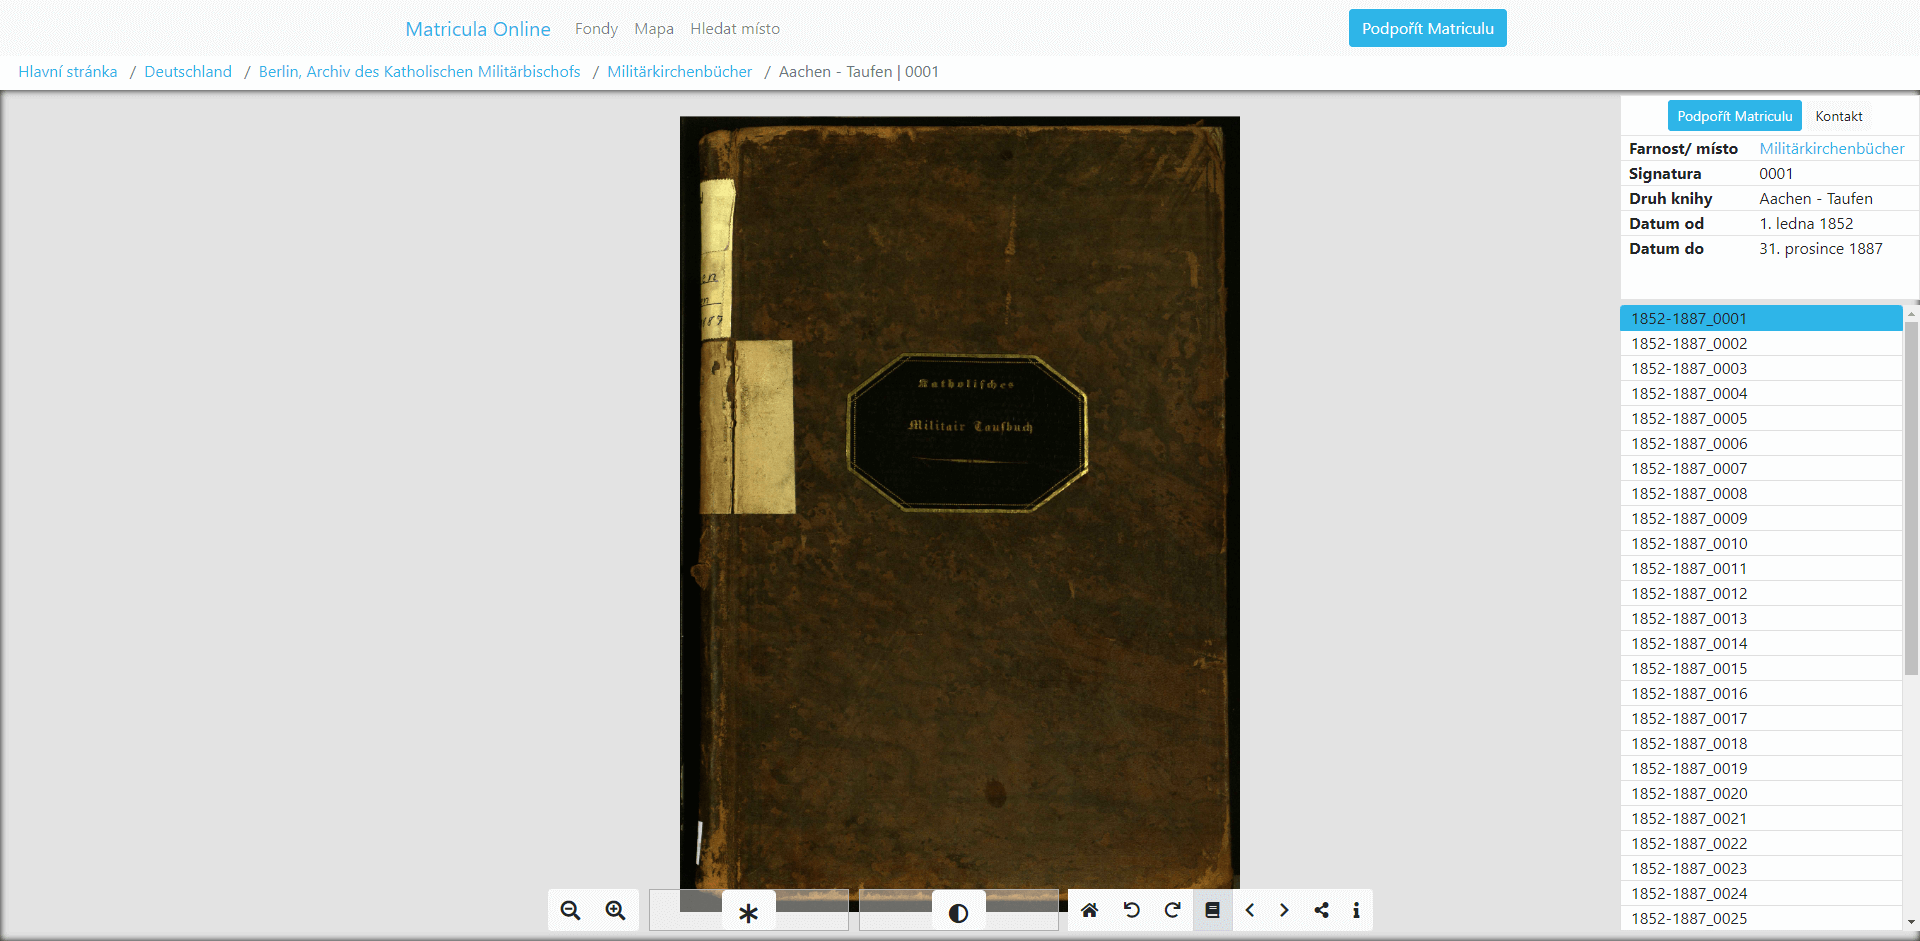
\includegraphics[scale=.2]{obrazky-figures/archives/matricula/prohlizec.png}
    \caption{Prohlížeč archiválií v~systému Matricula}
\end{figure}
\newpage

\section{Zhodnocení dostupných webových aplikací}
Po představení jednotlivých webových aplikací je nutné identifikovat jejich klíčové vlastnosti a sestavení seznamu vlastností, které by prohlížeč archiválií měl dle mého názoru obsahovat. Při prohlížení archiválií jsou preferovány systémy asynchronně načítající další stránky a kde~nedochází k~přenačtení celého rozhraní. Dalším důležitým aspektem je plocha rozhraní, jež jednotlivé systémy alokovaly pro samotné zobrazení archiválie. Za velmi důležitou vlastnost systému považuji režim zobrazení na celou obrazovku, během kterého musí být maximalizována plocha pro zobrazení dané archiválie.
\newpara
Za mandatorní prvky prohlížeče archiválií považuji ovládací panel a~náhled dalších snímků, což ne všechny systémy poskytovaly. Některé systémy umožňovaly efektivní práci pomocí předdefinovaných klávesových zkratek, avšak u~spousty systémů chyběla intuitivní nápověda, kde by se uživatel naučil se zkratkami rychle pracovat.
\newpara
Jelikož výsledná kvalita zdigitalizovaných skenů není konzistentní, tak je vhodné, aby prohlížeč umožňoval rotovat snímky o libovolný stupeň, což většina systémů neumožňovala. V systému ARON existuje archiválie, která je naskenována pod úhlem 45°, ale aplikace umožňuje rotovat archiválii pouze po 90°, což znemožňuje srovnat řádky textu do vodorovné polohy. Další kladnou vlastností některých systémů je možnost manuální úpravy jasu a~kontrastu skenů. Některé archiválie nejsou naskenovány v~čitelné podobě a~toto nastavení může v~mnoha případech zlepšit čitelnost. Při práci s~archiválií se uživatel často zaměřuje pouze na jistou část skenu, na níž má přiblíženo. Z tohoto důvodu má většina systémů funkci Zachovat zobrazení, která při změně skenu zachová aktuální přiblížení a~pozici v~rámci archiválie. V~rámci systému Actapublica byly definovány záložky, což usnadňovalo vyhledávání v~matrikách, kde mohou být záznamy z~více obcí. 
\newpara
Vyhledávání konkrétní archiválie se liší napříč systémy, které nabízejí různé možnosti od hledání podle určitých atributů až po plné textové vyhledávání. Velmi užitečná je funkce, kdy systém při našeptávání názvu obcí zobrazil také informaci o kraji a okrese. Tuto funkcionalitu ocení badatelé v případě, kdy existuje více obcí se stejným názvem a potřebují je od sebe odlišit.
\newpara
K jednoznačné identifikaci obce lze využít identifikátor RÚIAN \cite{coToJeRuian}. Registr územní identifikace adres a~nemovitostí je jedinečným identifikátorem v~rámci České republiky pro územní prvky, územní evidenční jednotky a adresy. Kromě jedinečné identifikace se dále RÚIAN používá k~určení jejich vlastníků a~zjištění podrobnějších informací o jednotlivých parcelách a~budovách. Celý informační systém spravuje Český úřad zeměměřický a~katastrální. Tento systém se kromě správy nemovitostí dále používá pro urbanismus a~územní plánování.
\newpara
Pro lepší přehlednost je plánovaná funkcionalita systému rozdělena do kategorií a~zaznamenána v~diagramu.
\begin{figure}[htbp]
\centering
    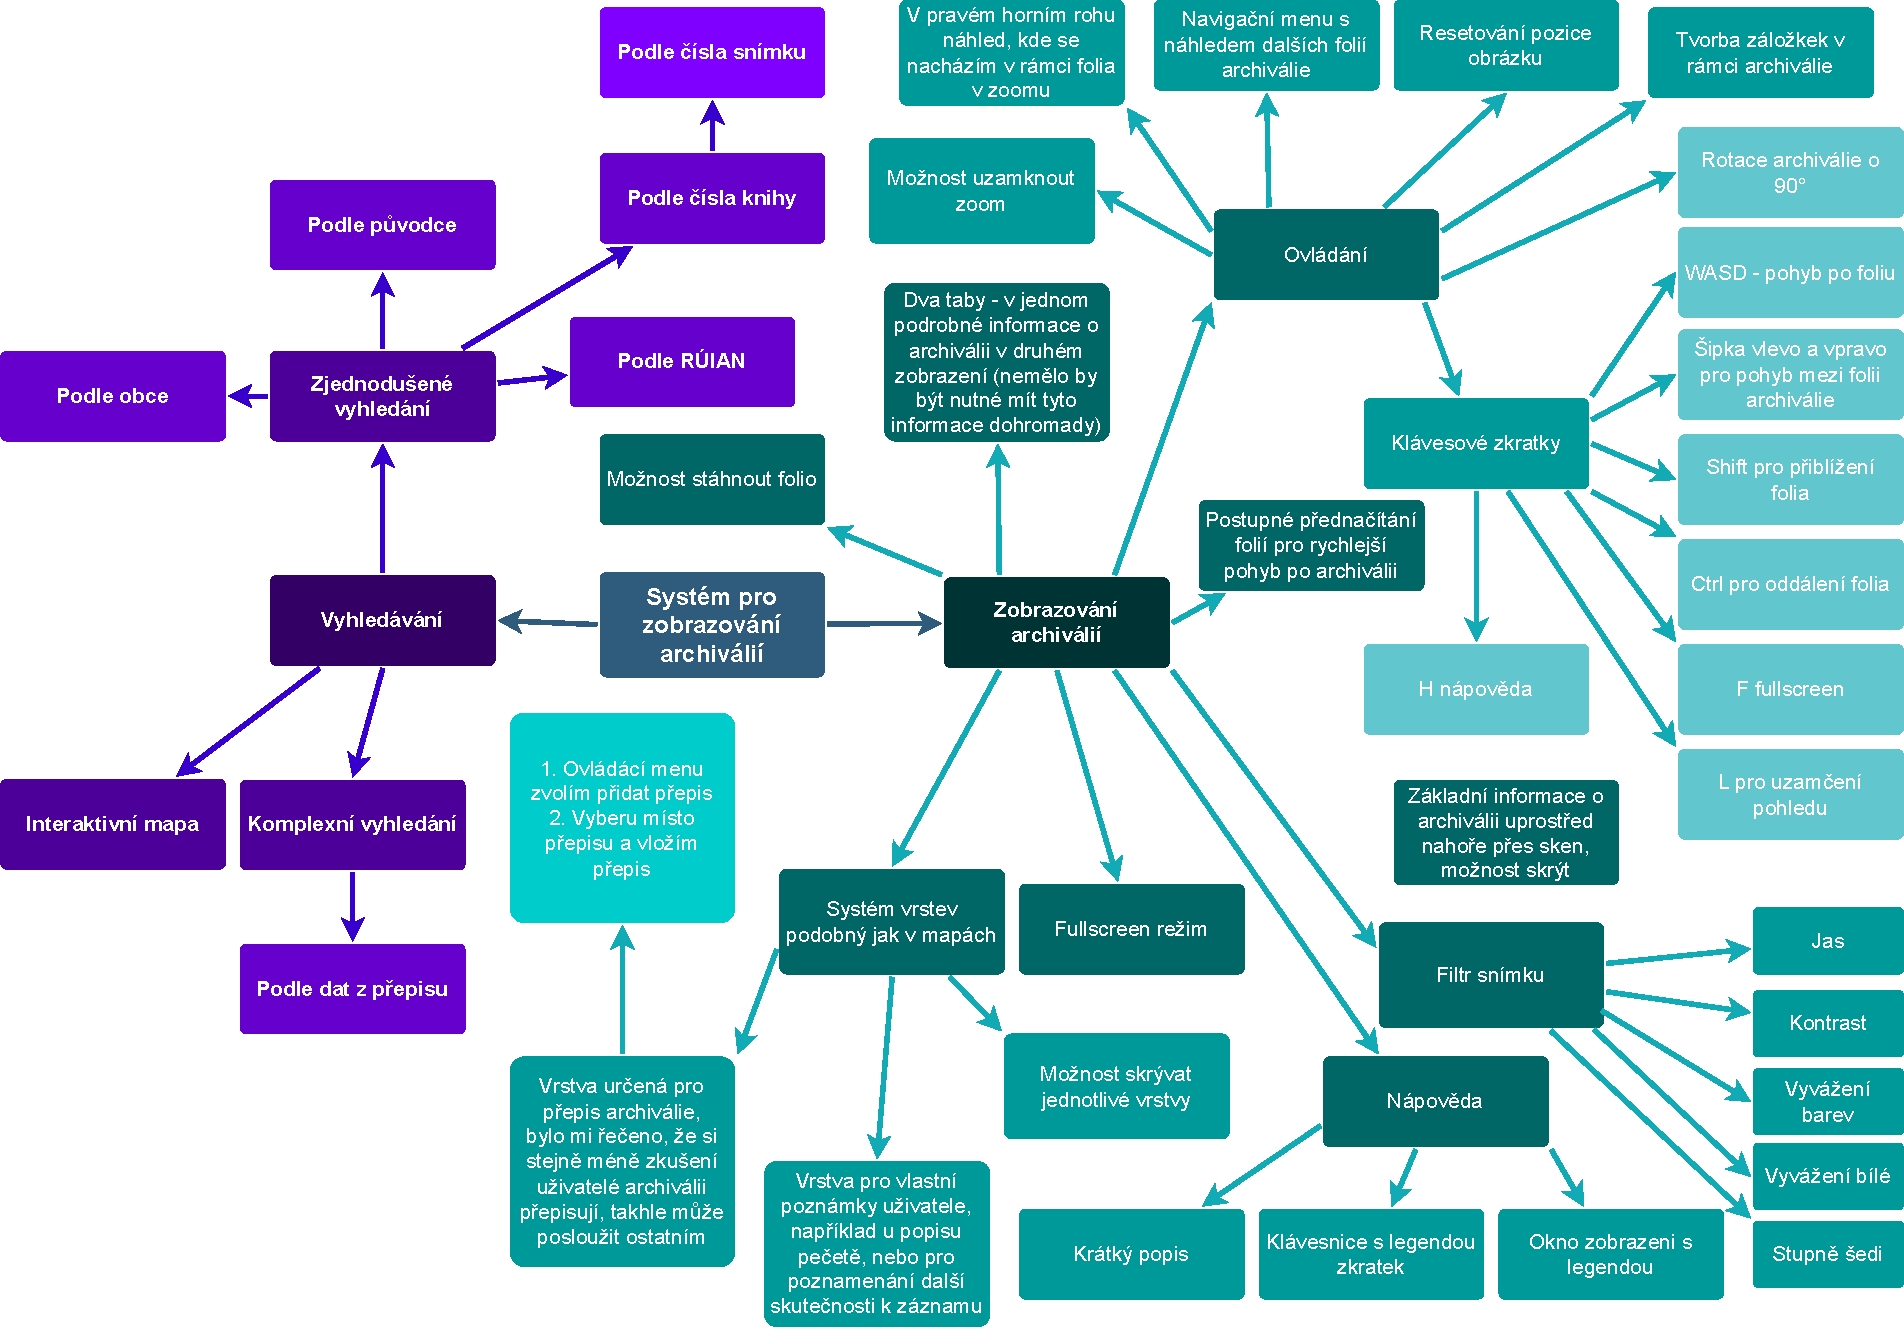
\includegraphics[scale=.45]{obrazky-figures/archives/functionality_diagram.pdf}
    \caption{Diagram funkcionality}
\end{figure}